\chapter{Probabilistic Circuits}
\label{ch:pc}

As we briefly mentioned in the last chapter, Probabilistic Circuits (PCs) are conceptualized as
computational graphs under special conditions. In this chapter, \Cref{sec:pc} to be more precise,
we formally define PCs and give an intuition on their syntax, viewing other probabilistic models
through the lenses of the PC framework. In \Cref{sec:const}, we describe the special structural
constraints that give PCs their inference power over other generative models and state which
queries (as far as we know) are enabled from each constraint.

\section{Distributions as Computational Graphs}
\label{sec:pc}

Probabilistic circuits are directed acyclic graphs usually recursively defined in terms of their
computational units. In its simplest form a PC is a single unit with no outgoing edges whose value
corresponds to the result of a function. These are often called \emph{input} nodes, and can take
any form as long as its value is tractably computable. More concretely, input nodes typically
represent probability density (or mass) functions, although they also support inputs as joint
probability density functions of complex non-parametric models as well. To simplify notation, from
here on out we shall use the term distribution and probability density (resp. mass) function
interchangeably and argue that the input node represents a probability distribution.
\begin{example}[sidebyside,lefthand width=0.6\textwidth]{Gaussians as probabilistic circuits}{gaussians} %
  Let $\Leaf_p$ an input node and $p(X)=\gaussian(X;\mu,\sigma^2)$ a univariate Gaussian
  distribution. Computing any query on $\Leaf_p$ is straightforward: any query on
  $\Leaf_p$ directly translates to $p$. As an example, suppose $\mu=0$ and $\sigma^2=1$ and
  we wish to compute $\Leaf_p(x=0.8)$. The probability of this input shall then be
  \begin{equation*}
    \Leaf_p(x=0.8)=\gaussian(x=0.8;\mu=0,\sigma^2=1)=0.29.
  \end{equation*}
  \tcblower
  \begin{center}
    \begin{tikzpicture}
      \pgfplotsset{
        every axis/.append style={
          axis line style={->},
          tick label style={font={\scriptsize\bfseries}},
          x tick label style={color=white,above right},
          y tick label style={color=white,above right},
          grid style={black,dashed},
        }
      }
      \begin{axis}[
        no markers, domain=-5:5, samples=35,
        height=2.75cm, width=\columnwidth,
        xtick={0.8}, ytick={0.29},
        xticklabels={\colorbox{boxblue}{\textbf{0.8}}},
        yticklabels={\colorbox{boxgreen}{\textbf{0.29}}},
        axis lines*=left, xlabel=$x$, ylabel=$p(x)$,
        every axis y label/.style={font=\scriptsize,at={(axis description cs:-0.1,0.9)},anchor=south},
        every axis x label/.style={font=\scriptsize,at=(current axis.right of origin),anchor=west},
        enlargelimits=false, clip=false, axis on top,
        grid = major
      ]
        \addplot[very thick,boxteal] {gauss(0,1)};
      \end{axis}
    \end{tikzpicture}

    \begin{tikzpicture}
      \node (x) at (0, 0) {$x$};
      \newGaussNode{g}{$(x) + (1,0)$};
      \node (px) at ($(g) + (1.25,0)$) {$p(x)$};
      \draw[boxdgray,edge] (x) -- (g);
      \draw[boxdgray,edge] (g) -- (px);

      \newGaussNode[label=below:$X$]{gv}{$(g) - (0,1.0)$};
      \node (xv) at ($(gv) - (1.25,0)$) {\colorbox{boxblue}{\color{white}$\mathbf{.80}$}};
      \node (pxv) at ($(gv) + (1.25,0)$) {\colorbox{boxgreen}{\color{white}$\mathbf{.29}$}};
      \draw[boxdgray,edge] (xv) -- (gv);
      \draw[boxdgray,edge] (gv) -- (pxv);
    \end{tikzpicture}
  \end{center}
\end{example}
Let $\Leaf_p$ a PC input node and denote $p$ as its inherent probability distribution. By
definition, any query $f:\mathcal{X}\to \mathcal{Y}$ which is tractable on $p$ is tractable on
$\Leaf_p$. We shall denote $\Leaf_p(\set{X})=p(\set{X})$, and often omit $p$ when its explicit form
is not needed. Evidently, a single input node lacks the expressivity for modeling complex models, otherwise we
would have just used the input distribution as a standalone model. The expressiveness of PCs comes
from recursively combining distributions into complex functions. This can be done through
computational units that either compute convex combinations or products of their children. Let us
first look at convex combinations, known in the literature as \emph{sum} nodes.

Let $\Sum$ be a PC sum node, and denote by $\Ch(\Sum)$ the children nodes of $\Sum$. For every edge
$\edge{\Sum\Child}$ coming out of $\Sum$ and going to $\Child$, we attribute a weight $w_{\Sum,
\Child}>0$, such that $\sum_{\Child\in\Ch(\Sum)} w_{\Sum,\Child} = 1$. A sum node semantically
defines a mixture model over its children, essentially acting as a latent variable over the
component distributions \citep{poon11,peharz16}. Its value is the weighted sum of its children
$p_{\Sum}(\set{X}=\set{x})=\sum_{\Child\in\Ch(\Sum)}w_{\Sum,\Child}\cdot
p_{\Child}(\set{X}=\set{x})$. To simplify notation, we shall use $\Node(\set{X}=\set{x})$ as an
alias for $p_{\Node}(\set{X}=\set{x})$, that is, the probability function given by $\Node$'s
induced distribution. We often omit the variable assignment $\set{X}=\set{x}$ to $\set{x}$ if the
notation is unambiguous.

\newcommand\mone{1}%
\newcommand\sone{0.65}%
\newcommand\mtwo{2.5}%
\newcommand\stwo{0.85}%
\newcommand\mthr{4}%
\newcommand\sthr{0.6}%
\begin{example}[sidebyside,lefthand width=0.55\textwidth]{Gaussian mixture models as probabilistic circuits}{mixgauss}
  A Gaussian Mixture Model (GMM) defines a mixture over Gaussian components. Say we wish to compute
  the probability of $X=x$ for a GMM $\mathcal{G}$ with three components
  $\gaussian_1(\mu_1=\mone,\sigma^2_1=\sone)$, $\gaussian_2(\mu_2=\mtwo, \sigma^2_1=\stwo)$ and
  $\gaussian_3(\mu_3=\mthr,\sigma^2_3=\sthr)$, and suppose we have weights set to
  $\phi=(0.4,0.25,0.35)$. Computing the probability of $G$ amounts to the weighted summation
  \begin{align*}
    \mathcal{G}(X=x)=&0.4\cdot\gaussian_1(x;\mu_1,\sigma^2_2)+0.25\cdot\gaussian_2(x;\mu_2,\sigma^2_2)+\\
                     &0.35\cdot\gaussian_3(x;\mu_3,\sigma^2_3),
  \end{align*}
  which is equivalent to a computational graph (i.e. a PC) with a sum node whose weights are set to
  $\phi$ and children are the components of the mixture. The figure on the right shows
  $\mathcal{G}$ (top) and its corresponding PC (middle). Given $x=1.5$ (in blue), input nodes are
  computed following the inference flow (bottom, gray edges) up to the root sum node (in red),
  where a weighted summation is computed to output the probability (in green).

  \tcblower
  \begin{center}
    \begin{tikzpicture}
      \pgfplotsset{
        every axis/.append style={
          axis line style={->},
          tick label style={font={\scriptsize\bfseries}},
          x tick label style={color=white,below},
          y tick label style={color=white,left},
          grid style={black,dashed},
        }
      }
      \begin{axis}[
        no markers, domain=-1:6, samples=35,
        height=3.75cm, width=\columnwidth,
        xtick={1.5}, ytick={0.2414},
        xticklabels={\colorbox{boxblue}{\textbf{1.5}}},
        yticklabels={\colorbox{boxgreen}{\textbf{0.24}}},
        axis lines*=left, xlabel=$x$, ylabel=$p(x)$,
        every axis y label/.style={font=\scriptsize,at={(axis description cs:-0.1,0.9)},anchor=south},
        every axis x label/.style={font=\scriptsize,at=(current axis.right of origin),anchor=west},
        enlargelimits=false, clip=false, axis on top,
        grid = major
      ]
        \path[name path=axis] (axis cs:0,0) -- (axis cs:5,0);
        \addplot[very thick,boxteal,name path=g1] {gauss(\mone,\sone)};
        \addplot[very thick,boxorange,name path=g2] {gauss(\mtwo,\stwo)};
        \addplot[very thick,boxpurple,name path=g3] {gauss(\mthr,\sthr)};
        \addplot[very thick,boxred] {mixgauss3(\mone,\sone,\mtwo,\stwo,\mthr,\sthr,0.4,0.25,0.35)};
        \addplot[boxteal!60] fill between [of=g1 and axis];
        \addplot[boxorange!50] fill between [of=g2 and axis];
        \addplot[boxpurple!40] fill between [of=g3 and axis];
        \node at (\mone, 0.7) {\tiny$\mu_1=\mone$};
        \node at (\mtwo, 0.5) {\tiny$\mu_2=\mtwo$};
        \node at (\mthr, 0.75) {\tiny$\mu_3=\mthr$};
      \end{axis}
    \end{tikzpicture}

    \begin{tikzpicture}
      \newSumNode[fill=boxred!70]{s}{0,0};
      \newGaussNode[fill=boxteal]{g1}{$(s) + (-1.5,-1)$};
      \newGaussNode[fill=boxorange!80]{g2}{$(s) + (0,-1)$};
      \newGaussNode[fill=boxpurple!60]{g3}{$(s) + (1.5,-1)$};
      \draw[edge] (s) edge (g1);
      \draw[edge] (s) edge (g2);
      \draw[edge] (s) edge (g3);
      \node at ($(s) + (-1.2,-0.35)$) {\scriptsize$.40$};
      \node at ($(s) + (-0.3,-0.5)$) {\scriptsize$.25$};
      \node at ($(s) + (1,-0.35)$) {\scriptsize$.35$};
      \node (l1) at ($(g1) + (0,-0.5)$) {\scriptsize$\gaussian_1(\mone,\sone)$};
      \node (l2) at ($(g2) + (0,-0.5)$) {\scriptsize$\gaussian_2(\mtwo,\stwo)$};
      \node (l3) at ($(g3) + (0,-0.5)$) {\scriptsize$\gaussian_3(\mthr,\sthr)$};
    \end{tikzpicture}

    \begin{tikzpicture}
      \newSumNode[fill=boxred!70]{s}{0,0};
      \newGaussNode[fill=boxteal]{g1}{$(s) + (-1.5,-1)$};
      \newGaussNode[fill=boxorange!80]{g2}{$(s) + (0,-1)$};
      \newGaussNode[fill=boxpurple!60]{g3}{$(s) + (1.5,-1)$};
      \draw[edge] (s) edge[bend right=5] (g1);
      \draw[edge] (s) edge[bend right=5] (g2);
      \draw[edge] (s) edge[bend right=5] (g3);
      \node at ($(s) + (-1.2,-0.35)$) {\scriptsize$.40$};
      \node at ($(s) + (-0.3,-0.5)$) {\scriptsize$.25$};
      \node at ($(s) + (1,-0.35)$) {\scriptsize$.35$};
      \node (inp) at ($(g2) + (0,-1.5)$) {\scriptsize\colorbox{boxblue}{\color{white}$\mathbf{1.5}$}};
      \node (out) at ($(s) + (0,1.0)$) {\scriptsize\colorbox{boxgreen}{\color{white}$\mathbf{0.24}$}};
      \draw[edge,boxdgray] (s) -- (out);
      \node (l1) at ($(g1) + (0,-0.5)$) {\scriptsize\colorbox{boxteal}{\color{white}$\mathbf{0.45}$}};
      \node (l2) at ($(g2) + (0,-0.5)$) {\scriptsize\colorbox{boxorange}{\color{white}$\mathbf{0.23}$}};
      \node (l3) at ($(g3) + (0,-0.5)$) {\scriptsize\colorbox{boxpurple!80}{\color{white}$\mathbf{0.00}$}};
      \draw[edge,boxdgray] (inp) edge (l1);
      \draw[edge,boxdgray] (inp) edge (l2);
      \draw[edge,boxdgray] (inp) edge (l3);
      \draw[edge,boxdgray] (g1) edge[bend left=-5] (s);
      \draw[edge,boxdgray] (g2) edge[bend left=-5] (s);
      \draw[edge,boxdgray] (g3) edge[bend left=-5] (s);
    \end{tikzpicture}
  \end{center}
\end{example}

So far, the only nonlinearities present in PCs come from the internal computations of input nodes.
In fact, a PC that only contains sums inputs can always be reduced to a sum node rooted PC with a
single layer, i.e. a mixture model (see \Cref{thm:summix}). Adding \emph{product nodes} as another
form of nonlinearity increases expressivity sufficiently for PCs to be capable of representing any
(discrete) probability distribution \citep{darwiche03,martens14,peharz15}. More importantly,
products semantically act as factorizations of their children, indicating an independence
relationship between variables from different children. In practice, product nodes are simply
products of their childrens' distribution: if $\Prod$ is a PC product node, then its value is given
by $\Prod(\set{X}=\set{x})=\prod_{\Child\in\Ch(\Prod)}\Child(\set{X}=\set{x})$.

\newcommand\xmone{2}%
\newcommand\xsone{0.5}%
\newcommand\xmtwo{4}%
\newcommand\xstwo{0.8}%
\newcommand\ymone{3}%
\newcommand\ysone{0.7}%
\newcommand\ymtwo{5}%
\newcommand\ystwo{0.4}%
\begin{example}[sidebyside,lefthand width=0.55\textwidth]{Factors as probabilistic circuits}{factors}
  Say we have two GMMs $\mathcal{G}_1$ and $\mathcal{G}_2$. The first is a mixture model over
  variable $X$, with component weights $\phi_1=(0.3,0.7)$ and gaussians
  $\gaussian_1(\mu_1=\xmone,\sigma_1=\xsone)$ and $\gaussian_2(\mu_2=\xmtwo,\sigma_2=\xstwo)$. The
  second is composed of $\gaussian_3(\mu_3=\ymone,\sigma_2=\ysone)$ and $\gaussian_4(\mu_4=\ymtwo,
  \sigma_2=\ystwo)$, both distributions over variable $Y$ and with weights $\phi_2=(0.6,0.4)$.

  Suppose $X\indep Y$, yet we wish to compute the joint probability of both $x$ and $y$. If
  $X\indep Y$, then $p(x,y)=p(x)p(y)=\mathcal{G}_1(x)\mathcal{G}_2(y)$, which corresponds to a
  factoring of mixtures. This is represented as a product node (in green) over the two mixture
  models (in red and purple). The resulting joint of this circuit is shown below.
\begin{tikzpicture}
  \pgfplotsset{
    every axis/.append style={
      axis line style={->},
      axis lines=center,
      grid style={black,dashed},
      x tick label style={color=white,below},
      y tick label style={color=white,right},
      z tick label style={color=white,left},
    }
  }
  \begin{axis}[
    no markers, width=0.9\columnwidth,
    xtick={2}, ytick={4}, ztick={0.035},
    xticklabels={\colorbox{boxblue}{\textbf{2}}},
    yticklabels={\colorbox{boxblue}{\textbf{4}}},
    zticklabels={\colorbox{boxgreen}{\textbf{0.035}}},
    xlabel=$x$, ylabel=$y$, zlabel={$p(x,y)$},
    axis lines*=left,
    xlabel style={anchor=north west},
    ylabel style={anchor=south west},
    zlabel style={anchor=south west},
    enlargelimits=false, clip=false, axis on top,
    grid = major
  ]
    \addplot3[
      surf, samples=50,
      domain=0.5:6.5,
      y domain=1:6
    ] {((0.3*exp(-((x-\xmone)^2)/(2*\xsone^2))/\xsone+0.7*exp(-((x-\xmtwo)^2)/(2*\xstwo^2))/\xstwo)/2.5066)*(((0.6*exp(-((y-\ymone)^2)/(2*\ysone^2))/\ysone+0.4*exp(-((y-\ymtwo)^2)/(2*\ystwo^2))/\ystwo)/2.5066))};
  \end{axis}
\end{tikzpicture}

  \tcblower
  \begin{center}
    \begin{tikzpicture}
      \pgfplotsset{
        every axis/.append style={
          axis line style={->},
          tick label style={font={\scriptsize\bfseries}},
          x tick label style={color=white,below},
          y tick label style={color=white,left},
          grid style={black,dashed},
        }
      }
      \begin{axis}[
        no markers, domain=0:7, samples=35,
        height=3.0cm, width=\columnwidth,
        xtick={2}, ytick={0.25},
        xticklabels={\colorbox{boxblue}{\textbf{2}}},
        yticklabels={\colorbox{boxred}{\textbf{0.25}}},
        axis lines*=left, xlabel=$x$, ylabel=$p(x)$,
        every axis y label/.style={font=\scriptsize,at={(axis description cs:-0.1,0.9)},anchor=south},
        every axis x label/.style={font=\scriptsize,at=(current axis.right of origin),anchor=west},
        enlargelimits=false, clip=false, axis on top,
        grid = major
      ]
        \path[name path=axis] (axis cs:0,0) -- (axis cs:7,0);
        \addplot[very thick,boxteal,name path=g1] {gauss(\xmone,\xsone)};
        \addplot[very thick,boxorange,name path=g2] {gauss(\xmtwo,\xstwo)};
        \addplot[very thick,boxred] {mixgauss2(\xmone,\xsone,\xmtwo,\xstwo,0.3,0.7)};
        \addplot[boxteal!60] fill between [of=g1 and axis];
        \addplot[boxorange!50] fill between [of=g2 and axis];
        \node at (axis cs:\xmone,{egauss(\xmone,\xsone,\xmone)+0.1}) {\tiny$\mu_1=\xmone$};
        \node at (axis cs:\xmtwo,{egauss(\xmtwo,\xstwo,\xmtwo)+0.1}) {\tiny$\mu_2=\xmtwo$};
      \end{axis}
    \end{tikzpicture}
    \begin{tikzpicture}
      \pgfplotsset{
        every axis/.append style={
          axis line style={->},
          tick label style={font={\scriptsize\bfseries}},
          x tick label style={color=white,below},
          y tick label style={color=white,left},
          grid style={black,dashed},
        }
      }
      \begin{axis}[
        no markers, domain=1:7, samples=50,
        height=3.0cm, width=\columnwidth,
        xtick={4}, ytick={0.14},
        xticklabels={\colorbox{boxblue}{\textbf{4}}},
        yticklabels={\colorbox{boxpurple}{\textbf{0.14}}},
        axis lines*=left, xlabel=$y$, ylabel=$p(y)$,
        every axis y label/.style={font=\scriptsize,at={(axis description cs:-0.1,0.9)},anchor=south},
        every axis x label/.style={font=\scriptsize,at=(current axis.right of origin),anchor=west},
        enlargelimits=false, clip=false, axis on top,
        grid = major
      ]
        \path[name path=axis] (axis cs:0,0) -- (axis cs:7,0);
        \addplot[very thick,boxpink,name path=g1] {gauss(\ymone,\ysone)};
        \addplot[very thick,boxgoldenrod,name path=g2] {gauss(\ymtwo,\ystwo)};
        \addplot[very thick,boxpurple] {mixgauss2(\ymone,\ysone,\ymtwo,\ystwo,0.6,0.4)};
        \addplot[boxpink!40] fill between [of=g1 and axis];
        \addplot[boxgoldenrod!50] fill between [of=g2 and axis];
        \node at (axis cs:\ymone,{egauss(\ymone,\ysone,\ymone)+0.1}) {\tiny$\mu_3=\ymone$};
        \node at (axis cs:\ymtwo,{egauss(\ymtwo,\ystwo,\ymtwo)+0.1}) {\tiny$\mu_4=\ymtwo$};
      \end{axis}
    \end{tikzpicture}
    \begin{tikzpicture}
      \newProdNode[fill=boxgreen]{r}{0,0};
      \newSumNode[fill=boxred!70]{p}{$(r) + (-1.25,-0.75)$};
      \newSumNode[fill=boxpurple!60]{q}{$(r) + (1.25,-0.75)$};
      \newGaussNode[fill=boxteal]{x1}{$(p) + (-0.6,-1)$};
      \newGaussNode[fill=boxorange!80]{x2}{$(p) + (0.65,-1)$};
      \newGaussNode[fill=boxpink!50]{y1}{$(q) + (-0.6,-1)$};
      \newGaussNode[fill=boxgoldenrod!70]{y2}{$(q) + (0.6,-1)$};
      \draw[edge] (r) edge (p);
      \draw[edge] (r) edge (q);
      \draw[edge] (p) edge (x1);
      \draw[edge] (p) edge (x2);
      \draw[edge] (q) edge (y1);
      \draw[edge] (q) edge (y2);
      \node at ($(p) + (-0.5,-0.4)$) {\scriptsize$.3$};
      \node at ($(p) + (0.5,-0.4)$) {\scriptsize$.7$};
      \node at ($(q) + (-0.5,-0.4)$) {\scriptsize$.6$};
      \node at ($(q) + (0.5,-0.4)$) {\scriptsize$.4$};
      \node (l1) at ($(x1) + (0,-0.5)$) {\scriptsize$\gaussian_1(\xmone,\xsone)$};
      \node (l2) at ($(x2) + (0,-0.5)$) {\scriptsize$\gaussian_2(\xmtwo,\xstwo)$};
      \node (l3) at ($(y1) + (0,-0.5)$) {\scriptsize$\gaussian_1(\ymone,\ysone)$};
      \node (l4) at ($(y2) + (0,-0.5)$) {\scriptsize$\gaussian_2(\ymtwo,\ystwo)$};
    \end{tikzpicture}
    \begin{tikzpicture}
      \newProdNode[fill=boxgreen]{r}{0,0};
      \newSumNode[fill=boxred!70]{p}{$(r) + (-1.25,-0.75)$};
      \newSumNode[fill=boxpurple!60]{q}{$(r) + (1.25,-0.75)$};
      \newGaussNode[fill=boxteal]{x1}{$(p) + (-0.6,-1)$};
      \newGaussNode[fill=boxorange!80]{x2}{$(p) + (0.65,-1)$};
      \newGaussNode[fill=boxpink!50]{y1}{$(q) + (-0.6,-1)$};
      \newGaussNode[fill=boxgoldenrod!70]{y2}{$(q) + (0.6,-1)$};
      \draw[edge] (r) edge[bend right=5] (p);
      \draw[edge] (r) edge[bend right=5] (q);
      \draw[edge] (p) edge[bend right=5] (x1);
      \draw[edge] (p) edge[bend right=5] (x2);
      \draw[edge] (q) edge[bend right=5] (y1);
      \draw[edge] (q) edge[bend right=5] (y2);
      \node at ($(p) + (-0.5,-0.4)$) {\scriptsize$.3$};
      \node at ($(p) + (0.5,-0.4)$) {\scriptsize$.7$};
      \node at ($(q) + (-0.5,-0.4)$) {\scriptsize$.6$};
      \node at ($(q) + (0.5,-0.4)$) {\scriptsize$.4$};
      \node (l1) at ($(x1) + (0,-0.5)$) {\scriptsize\colorbox{boxteal}{\color{white}$\mathbf{0.24}$}};
      \node (l2) at ($(x2) + (0,-0.5)$) {\scriptsize\colorbox{boxorange}{\color{white}$\mathbf{0.01}$}};
      \node (l3) at ($(y1) + (0,-0.5)$) {\scriptsize\colorbox{boxpink}{\color{white}$\mathbf{0.12}$}};
      \node (l4) at ($(y2) + (0,-0.5)$) {\scriptsize\colorbox{boxgoldenrod}{\color{white}$\mathbf{0.01}$}};
      \draw[edge,boxdgray] (p) edge[bend left=-5] (r);
      \draw[edge,boxdgray] (q) edge[bend left=-5] (r);
      \draw[edge,boxdgray] (x1) edge[bend left=-5] (p);
      \draw[edge,boxdgray] (x2) edge[bend left=-5] (p);
      \draw[edge,boxdgray] (y1) edge[bend left=-5] (q);
      \draw[edge,boxdgray] (y2) edge[bend left=-5] (q);
      \node at ($(p) + (-0.3,0.6)$) {\scriptsize\colorbox{boxred}{\color{white}$\mathbf{0.25}$}};
      \node at ($(q) + (0.3,0.6)$) {\scriptsize\colorbox{boxpurple}{\color{white}$\mathbf{0.14}$}};
      \node (x) at ($(p) + (0,-2.5)$) {\scriptsize\colorbox{boxblue}{\color{white}$\mathbf{x=2}$}};
      \node (y) at ($(q) + (0,-2.5)$) {\scriptsize\colorbox{boxblue}{\color{white}$\mathbf{y=4}$}};
      \draw[edge,boxdgray] (x) edge (l1);
      \draw[edge,boxdgray] (x) edge (l2);
      \draw[edge,boxdgray] (y) edge (l3);
      \draw[edge,boxdgray] (y) edge (l4);
      \node (out) at ($(r) + (0,0.9)$) {\scriptsize\colorbox{boxgreen}{\color{white}$\mathbf{0.035}$}};
      \draw[edge,boxdgray] (r) edge (out);
    \end{tikzpicture}
  \end{center}
\end{example}

Now that we have introduced the three most important computational units in PCs, we are finally
ready to formally define probabilistic circuits.

\begin{definition}[Probabilistic circuit]
  A probabilistic circuits $\mathcal{C}$ is a rooted connected DAG whose nodes compute any
  tractable operation of their children, usually either convex combinations, known as \emph{sum}
  nodes, or \emph{products}. Nodes with no outgoing edges, i.e. \emph{input} nodes, are tractable
  nonnegative functions whose integrals exist and equal to one. Computing a value from
  $\mathcal{C}$ amounts to a bottom-up feedforward pass from input nodes to root. \label{def:pc}
\end{definition}

While we assume that \emph{tractable} operation or function is acceptable, we are usually
interested in $\bigo(1)$ time computable operations, and often assume the same of input functions
to simplify analysis. Further, in this dissertation we are only interested in convex combinations
and products, and as such only these operations are considered. When a probabilistic circuit
$\mathcal{C}$ contains no consecutive sums or products (i.e. for every sum all of its children are
either inputs or products and respectively for products) then it is said to be a \emph{standard}
form circuit. Any PC can be transformed into a \emph{standardized} circuit, a process we call
\emph{standardization} (see \Cref{thm:standard}).

\begin{remark}[breakable]{On operators and tractability}{optract}
  Throughout this work we consider only products and convex combinations (apart from the implicit
  operations contained within input nodes) as potential computational units. The question of whether
  any other operator could be used to gain expressivity without loss of tractability is without a
  doubt an interesting research question, and one that is actively being pursued. However, this is
  certainly out of the scope of this dissertation, and so we restrict discussion on this topic and
  only give a brief comment on operator tractability here, pointing to existing literature in this
  area of research.

  \citet{friesen16} formalize the notion of replacing sums and products in PCs with any pair of
  operators in a commutative semiring, giving results on the conditions for marginalization to be
  tractable. They provide examples of common semirings and to which known formalisms they
  correspond to. One such example are PCs under the Boolean semiring $(\{0,1\},\vee,\wedge,0,1)$
  for logical inference, which are equivalent to Negation Normal Form (NNF, \cite{barwise82}) and
  constitute an instance of Logic Circuits (LCs), of which Sentential Decision Diagrams (SDDs,
  \cite{darwiche11}) and Binary Decision Diagrams (BDDs, \cite{akers78}) are a part of. Another
  less common semiring in PCs is the real min-sum semiring $(\mathbb{R}_{\infty}, \min,+,\infty,0)$
  for nonconvex optimization \citep{friesen15}.

  Recently, \citet{vergari21} extensively covered tractability conditions and complexity bounds for
  convex combinations, products, $\exp$ (and more generally powers in both naturals and reals),
  quotients and logarithms, even giving results for complex information-theoretic queries, such as
  entropies and divergences. Notably, they analyze whether structural constraints (and thus, in a
  sense, tractability) under these conditions are preserved.

  Up to now, we have only considered summations as nonnegative weighted sums. Indeed, in most
  literature the sum node is defined as a convex combination. However, negative weights have
  appeared in Logistic Circuits \citep{liang19} for discriminative modeling; and in Probabilistic
  Generating Circuits \citep{zhang21}, a class of tractable probabilistic models that subsume PCs.
  \citet{maua17a} extend (nonnegative) weights in sum nodes with probability intervals, effectively
  inducing a credal set \citep{cozman00} for measuring imprecision.

  Other works include PCs with quotients \citep{sharir18a}, transformations \citep{pevny20a}, max
  \citep{melibari16}, and einsum \citep{peharz20b} operations.
\end{remark}

Before we address the key components that make PCs interesting tractable
probabilistic models, we must first discuss some important concepts that often come up in PC
literature. Mainly, we are interested in defining two notions here: the scope of a unit and induced
subcircuits.

In simple terms, the scope of a computational unit $\Node$ of a PC is merely the set of all
variables that appear in the descendants of $\Node$. More formally, denote by $\Sc(\Node)$
the set of all variables that appear in $\Node$.  We inductively compute the scope of circuit by a
bottom-up approach: the scope of an input node $\Leaf_p$ is the set of variables that appear in
$p$'s distribution\footnote{Although we previously defined input nodes as mere functions, here we
are explicitly associating a random variable to a \emph{probability} function. Indeed, if we
are being rigorous, we should define input nodes as a pair of random variable and function. To save
space we instead assume, as previously stated, that the function is seen as both the probability
(density) function as well as the distribution itself, and thus its scope is the scope of its
distribution, i.e. the random variables that come into play in a probability distribution.}, and
the scope of any other node is the union of all of its childrens' scopes.  The notion of scope is
essential to the structural constraints seen in \Cref{sec:const}.

As an example, take the circuit from \Cref{eg:factors}. The scope of input nodes
\inode[fill=boxteal]{\newGaussNode} and \inode[fill=boxorange!80]{\newGaussNode} are
$\Sc(\inode[fill=boxteal]{\newGaussNode})=\Sc(\inode[fill=boxorange!80]{\newGaussNode})=\{X\}$,
while $\Sc(\inode[fill=boxpink!50]{\newGaussNode})=\Sc(\inode[fill=boxgoldenrod!70]{\newGaussNode})
=\{Y\}$. Consequentially, their parent sum nodes will have the same scope as their children
$\Sc(\inode[fill=boxred!70]{\newSumNode})=\{X\}$ and $\Sc(\inode[fill=boxpurple!60]{\newSumNode})=
\{Y\}$, yet the root node's scope is $\Sc(\inode[fill=boxgreen]{\newProdNode})=\{X,Y\}$, since its
childrens' scopes are distinct. The size of a probabilistic circuit is the number of nodes and
edges of its computational graph. We use $|\mathcal{C}|$ to denote the size of a probabilistic
circuit $\mathcal{C}$.

Let $\mathcal{C}$ a probabilistic circuit and node $\Node\in\mathcal{C}$. We say that
$\mathcal{S}_{\Node}$ is a subcircuit of $\mathcal{C}$ rooted at $\Node$ if $\mathcal{S}_{\Node}$'s
root is $\Node$, all nodes and edges in $\mathcal{S}_{\Node}$ are also in $\mathcal{C}$ and
$\mathcal{S}$ is also a probabilistic circuit. We now introduce the concept of induced subcircuits
\citep{chan06,dennis15,peharz14}.

\begin{definition}[Induced subcircuit]
  Let $\mathcal{C}$ a probabilistic circuit. An induced subcircuit $\mathcal{S}$ of $\mathcal{C}$
  is a subcircuit of $\mathcal{C}$ rooted at $\mathcal{C}$'s root such that all edges coming out of
  product nodes in $\mathcal{C}$ are also in $\mathcal{S}$, and of all edges coming out of sum
  nodes in $\mathcal{C}$, only one is in $\mathcal{S}$.
\end{definition}

\begin{figure}[t]
  \begin{subfigure}[t]{0.245\textwidth}
    \begin{center}
      \resizebox{\textwidth}{!}{
      \begin{tikzpicture}
        \newSumNode[fill=boxgreen]{r}{0,0};
        \newProdNode[fill=boxred!70]{p1}{$(r) + (-1.5,-1)$};
        \newProdNode[fill=boxred!70]{p2}{$(r) + (0,-1)$};
        \newProdNode[fill=boxred!70]{p3}{$(r) + (1.5,-1)$};
        \newSumNode[fill=boxpurple!60]{s1}{$(p2) + (-2.0,-1)$};
        \newSumNode[fill=boxpurple!60]{s2}{$(p2) + (-0.66,-1)$};
        \newSumNode[fill=boxpurple!60]{s3}{$(p2) + (0.66,-1)$};
        \newSumNode[fill=boxpurple!60]{s4}{$(p2) + (2.0,-1)$};
        \newGaussNode[fill=boxteal]{g1}{$(s1) + (0,-1)$};
        \newGaussNode[fill=boxorange!80]{g2}{$(s2) + (0,-1)$};
        \newGaussNode[fill=boxpink!50]{g3}{$(s3) + (0,-1)$};
        \newGaussNode[fill=boxgoldenrod!70]{g4}{$(s4) + (0,-1)$};
        \draw[edge] (r) edge (p1);
        \draw[edge] (r) edge (p2);
        \draw[edge] (r) edge (p3);
        \draw[edge] (p1) edge (s1);
        \draw[edge] (p1) edge (s3);
        \draw[edge] (p2) edge (s2);
        \draw[edge] (p2) edge (s3);
        \draw[edge] (p3) edge (s2);
        \draw[edge] (p3) edge (s4);
        \draw[edge] (s1) edge (g1);
        \draw[edge] (s1) edge (g2);
        \draw[edge] (s2) edge (g1);
        \draw[edge] (s2) edge (g2);
        \draw[edge] (s3) edge (g3);
        \draw[edge] (s3) edge (g4);
        \draw[edge] (s4) edge (g3);
        \draw[edge] (s4) edge (g4);
      \end{tikzpicture}
      }
    \end{center}
    \caption{}
    \label{fig:pc}
  \end{subfigure}
  \begin{subfigure}[t]{0.245\textwidth}
    \begin{center}
      \resizebox{\textwidth}{!}{
      \begin{tikzpicture}
        \newSumNode[fill=boxgreen]{r}{0,0};
        \newProdNode[fill=boxred!70]{p1}{$(r) + (-1.5,-1)$};
        \newProdNode[fill=boxred!70]{p2}{$(r) + (0,-1)$};
        \newProdNode[fill=boxred!70]{p3}{$(r) + (1.5,-1)$};
        \newSumNode[fill=boxpurple!60]{s1}{$(p2) + (-2.0,-1)$};
        \newSumNode[fill=boxpurple!60]{s2}{$(p2) + (-0.66,-1)$};
        \newSumNode[fill=boxpurple!60]{s3}{$(p2) + (0.66,-1)$};
        \newSumNode[fill=boxpurple!60]{s4}{$(p2) + (2.0,-1)$};
        \newGaussNode[fill=boxteal]{g1}{$(s1) + (0,-1)$};
        \newGaussNode[fill=boxorange!80]{g2}{$(s2) + (0,-1)$};
        \newGaussNode[fill=boxpink!50]{g3}{$(s3) + (0,-1)$};
        \newGaussNode[fill=boxgoldenrod!70]{g4}{$(s4) + (0,-1)$};
        \draw[thick,red,edge] (r) edge (p1);
        \draw[boxgray,edge] (r) edge (p2);
        \draw[boxgray,edge] (r) edge (p3);
        \draw[thick,red,edge] (p1) edge (s1);
        \draw[thick,red,edge] (p1) edge (s3);
        \draw[boxgray,edge] (p2) edge (s2);
        \draw[boxgray,edge] (p2) edge (s3);
        \draw[boxgray,edge] (p3) edge (s2);
        \draw[boxgray,edge] (p3) edge (s4);
        \draw[thick,red,edge] (s1) edge (g1);
        \draw[boxgray,edge] (s1) edge (g2);
        \draw[boxgray,edge] (s2) edge (g1);
        \draw[boxgray,edge] (s2) edge (g2);
        \draw[thick,red,edge] (s3) edge (g3);
        \draw[boxgray,edge] (s3) edge (g4);
        \draw[boxgray,edge] (s4) edge (g3);
        \draw[boxgray,edge] (s4) edge (g4);
      \end{tikzpicture}
      }
    \end{center}
  \end{subfigure}\begin{subfigure}[t]{0.245\textwidth}
    \begin{center}
      \resizebox{\textwidth}{!}{
      \begin{tikzpicture}
        \newSumNode[fill=boxgreen]{r}{0,0};
        \newProdNode[fill=boxred!70]{p1}{$(r) + (-1.5,-1)$};
        \newProdNode[fill=boxred!70]{p2}{$(r) + (0,-1)$};
        \newProdNode[fill=boxred!70]{p3}{$(r) + (1.5,-1)$};
        \newSumNode[fill=boxpurple!60]{s1}{$(p2) + (-2.0,-1)$};
        \newSumNode[fill=boxpurple!60]{s2}{$(p2) + (-0.66,-1)$};
        \newSumNode[fill=boxpurple!60]{s3}{$(p2) + (0.66,-1)$};
        \newSumNode[fill=boxpurple!60]{s4}{$(p2) + (2.0,-1)$};
        \newGaussNode[fill=boxteal]{g1}{$(s1) + (0,-1)$};
        \newGaussNode[fill=boxorange!80]{g2}{$(s2) + (0,-1)$};
        \newGaussNode[fill=boxpink!50]{g3}{$(s3) + (0,-1)$};
        \newGaussNode[fill=boxgoldenrod!70]{g4}{$(s4) + (0,-1)$};
        \draw[boxgray,edge] (r) edge (p1);
        \draw[thick,blue,edge] (r) edge (p2);
        \draw[boxgray,edge] (r) edge (p3);
        \draw[boxgray,edge] (p1) edge (s1);
        \draw[boxgray,edge] (p1) edge (s3);
        \draw[thick,blue,edge] (p2) edge (s2);
        \draw[thick,blue,edge] (p2) edge (s3);
        \draw[boxgray,edge] (p3) edge (s2);
        \draw[boxgray,edge] (p3) edge (s4);
        \draw[boxgray,edge] (s1) edge (g1);
        \draw[boxgray,edge] (s1) edge (g2);
        \draw[boxgray,edge] (s2) edge (g1);
        \draw[thick,blue,edge] (s2) edge (g2);
        \draw[boxgray,edge] (s3) edge (g3);
        \draw[thick,blue,edge] (s3) edge (g4);
        \draw[boxgray,edge] (s4) edge (g3);
        \draw[boxgray,edge] (s4) edge (g4);
      \end{tikzpicture}
      }
    \end{center}
    \caption{}
    \label{fig:subcircs}
  \end{subfigure}\begin{subfigure}[t]{0.245\textwidth}
    \begin{center}
      \resizebox{\textwidth}{!}{
      \begin{tikzpicture}
        \newSumNode[fill=boxgreen]{r}{0,0};
        \newProdNode[fill=boxred!70]{p1}{$(r) + (-1.5,-1)$};
        \newProdNode[fill=boxred!70]{p2}{$(r) + (0,-1)$};
        \newProdNode[fill=boxred!70]{p3}{$(r) + (1.5,-1)$};
        \newSumNode[fill=boxpurple!60]{s1}{$(p2) + (-2.0,-1)$};
        \newSumNode[fill=boxpurple!60]{s2}{$(p2) + (-0.66,-1)$};
        \newSumNode[fill=boxpurple!60]{s3}{$(p2) + (0.66,-1)$};
        \newSumNode[fill=boxpurple!60]{s4}{$(p2) + (2.0,-1)$};
        \newGaussNode[fill=boxteal]{g1}{$(s1) + (0,-1)$};
        \newGaussNode[fill=boxorange!80]{g2}{$(s2) + (0,-1)$};
        \newGaussNode[fill=boxpink!50]{g3}{$(s3) + (0,-1)$};
        \newGaussNode[fill=boxgoldenrod!70]{g4}{$(s4) + (0,-1)$};
        \draw[boxgray,edge] (r) edge (p1);
        \draw[boxgray,edge] (r) edge (p2);
        \draw[thick,green!20!black,edge] (r) edge (p3);
        \draw[boxgray,edge] (p1) edge (s1);
        \draw[boxgray,edge] (p1) edge (s3);
        \draw[boxgray,edge] (p2) edge (s2);
        \draw[boxgray,edge] (p2) edge (s3);
        \draw[thick,green!20!black,edge] (p3) edge (s2);
        \draw[thick,green!20!black,edge] (p3) edge (s4);
        \draw[boxgray,edge] (s1) edge (g1);
        \draw[boxgray,edge] (s1) edge (g2);
        \draw[thick,green!20!black,edge] (s2) edge (g1);
        \draw[boxgray,edge] (s2) edge (g2);
        \draw[boxgray,edge] (s3) edge (g3);
        \draw[boxgray,edge] (s3) edge (g4);
        \draw[boxgray,edge] (s4) edge (g3);
        \draw[thick,green!20!black,edge] (s4) edge (g4);
      \end{tikzpicture}
      }
    \end{center}
  \end{subfigure}
  \caption{A probabilistic circuit (a) and 3 of the 12 possible induced subcircuits (b).}
  \label{fig:induced}
\end{figure}

Examples of induced subcircuits are visualized in \Cref{fig:induced}. When the induced subcircuit
is a tree, as is the case in \Cref{fig:induced}, they are referred to as induced tree
\citep{zhao15,zhao16b}.

So far, by \Cref{def:pc} a PC does not yet necessarily represent a probability distribution with
tractable (marginal) inference. In the next section, we formally define sufficient conditions for
tractability in the form of structural constraints that we have only previously mentioned in
passing.

\section{Deciding What to Constraint}
\label{sec:const}

In this section we are interested in studying how the structural constraints in PCs enable
different inference tasks. We shall first cover the more basic queries, namely \emph{probability of
evidence} (\evi), \emph{marginal probability} (\mar), \emph{conditional probability} (\con) and
\emph{maximum a posteriori probability} (\map). After that we briefly address more complex queries
such as mutual information, entropies and \emph{expectation} (\expc).

\subsection{Basic Queries}

The most basic inference task we are interested in computing is the probability of evidence. To
unlock this, we must introduce two structural constraints known as \emph{smoothness} and
\emph{decomposability}.

\begin{definition}[Smoothness]
  A probabilistic circuit $\mathcal{C}$ is said to be \emph{smooth} if for every sum node $\Sum$ in
  $\mathcal{C}$, $\Sc(\Child_1)=\Sc(\Child_2)$ for $\Child_1,\Child_2\in\Ch(\Sum)$.
\end{definition}

\begin{definition}[Decomposability]
  A probabilistic circuit $\mathcal{C}$ is said to be \emph{decomposable} if for every product node
  $\Prod$ in $\mathcal{C}$, $\Sc(\Child_1)\cap\Sc(\Child_2)=\emptyset$ for $\Child_1,\Child_2\in
  \Ch(\Prod)$.
\end{definition}

When a PC is \emph{decomposable}, all of its induced subcircuits are induced trees. For any
\emph{smooth} and \emph{decomposable} PC, computing \evi{} is done in linear time in the number of
edges. In fact this is true for \mar{} and \con{} as well. To compute marginals, it is sufficient
to compute the corresponding marginals with respect to each input node and proceed to propagate
values bottom-up. For conditionals, we simply compute two passes: one where we marginalize the
conditional variables and the other any other variables that are not present in our query. These
procedures are formalized in the theorem below.

\begin{restatable}[\cite{poon11,pclec,vergari21}]{theorem}{linevi}
  \label{thm:linevi}
  Let $\mathcal{C}$ a \emph{smooth} and \emph{decomposable} PC. Any one of \evi{}, \mar{} or \con{}
  can be computed in linear time (in the number of edges of $\mathcal{C}$).
\end{restatable}

\begin{figure}[t]
  \begin{subfigure}[t]{0.31\textwidth}
    \begin{center}
      \begin{tikzpicture}
        \newSumNode[fill=boxgreen]{r}{0,0};
        \newProdNode[fill=boxred]{p1}{$(r) + (-1.5,-1)$};
        \newProdNode[fill=boxred]{p2}{$(r) + (0,-1)$};
        \newProdNode[fill=boxred]{p3}{$(r) + (1.5,-1)$};
        \newGaussNode[fill=boxteal,label=below:{$A$}]{a}{$(p1) + (0,-1)$};
        \newGaussNode[fill=boxorange!80,label=below:{$B$}]{b}{$(p2) + (0,-1)$};
        \newGaussNode[fill=boxpink!50,label=below:{$C$}]{c}{$(p3) + (0,-1)$};
        \draw[edge] (r) edge (p1);
        \draw[edge] (r) edge (p2);
        \draw[edge] (r) edge (p3);
        \draw[edge] (p1) edge (a);
        \draw[edge] (p1) edge (b);
        \draw[edge] (p2) edge (a);
        \draw[edge] (p2) edge (c);
        \draw[edge] (p3) edge (b);
        \draw[edge] (p3) edge (c);
      \end{tikzpicture}
    \end{center}
    \caption{}
  \end{subfigure}
  \begin{subfigure}[t]{0.31\textwidth}
    \begin{center}
      \begin{tikzpicture}
        \newProdNode[fill=boxgreen]{r}{0,0};
        \newSumNode[fill=boxred!70]{p1}{$(r) + (-2.0,-1)$};
        \newSumNode[fill=boxred!70]{p2}{$(r) + (-0.66,-1)$};
        \newSumNode[fill=boxred!70]{p3}{$(r) + (0.66,-1)$};
        \newSumNode[fill=boxred!70]{p4}{$(r) + (2.0,-1)$};
        \newGaussNode[fill=boxteal,label=below:{$A$}]{a1}{$(p1) + (0,-1)$};
        \newGaussNode[fill=boxteal,label=below:{$A$}]{a2}{$(p2) + (0,-1)$};
        \newGaussNode[fill=boxorange!80,label=below:{$B$}]{b1}{$(p3) + (0,-1)$};
        \newGaussNode[fill=boxorange!80,label=below:{$B$}]{b2}{$(p4) + (0,-1)$};
        \draw[edge] (r) -- (p1);
        \draw[edge] (r) -- (p2);
        \draw[edge] (r) -- (p3);
        \draw[edge] (r) -- (p4);
        \draw[edge] (p1) -- (a1);
        \draw[edge] (p1) -- (a2);
        \draw[edge] (p2) -- (a1);
        \draw[edge] (p2) -- (a2);
        \draw[edge] (p3) -- (b1);
        \draw[edge] (p3) -- (b2);
        \draw[edge] (p4) -- (b1);
        \draw[edge] (p4) -- (b2);
      \end{tikzpicture}
    \end{center}
    \caption{}
  \end{subfigure}
  \begin{subfigure}[t]{0.31\textwidth}
    \begin{center}
      \begin{tikzpicture}
        \newProdNode[fill=boxgreen]{r}{0,0};
        \newSumNode[fill=boxred!70]{s1}{$(r) + (-1.0,-0.5)$};
        \newSumNode[fill=boxred!70]{s2}{$(r) + (1.0,-0.5)$};
        \newProdNode[fill=boxpurple!60]{p1}{$(s1) + (-0.5,-0.75)$};
        \newProdNode[fill=boxpurple!60]{p2}{$(s1) + (0.5,-0.75)$};
        \newProdNode[fill=boxpurple!60]{p3}{$(s2) + (-0.5,-0.75)$};
        \newProdNode[fill=boxpurple!60]{p4}{$(s2) + (0.5,-0.75)$};
        \newGaussNode[fill=boxteal,label=below:{$A$}]{a}{$(p1) + (0,-0.75)$};
        \newGaussNode[fill=boxorange!80,label=below:{$B$}]{b}{$(p2) + (0,-0.75)$};
        \newGaussNode[fill=boxpink!50,label=below:{$C$}]{c}{$(p3) + (0,-0.75)$};
        \newGaussNode[fill=boxgoldenrod!70,label=below:{$D$}]{d}{$(p4) + (0,-0.75)$};
        \draw[edge] (r) -- (s1);
        \draw[edge] (r) -- (s2);
        \draw[edge] (s1) -- (p1);
        \draw[edge] (s1) -- (p2);
        \draw[edge] (s2) -- (p3);
        \draw[edge] (s2) -- (p4);
        \draw[edge] (p1) -- (a);
        \draw[edge] (p1) -- (b);
        \draw[edge] (p2) -- (a);
        \draw[edge] (p2) -- (b);
        \draw[edge] (p3) -- (c);
        \draw[edge] (p3) -- (d);
        \draw[edge] (p4) -- (c);
        \draw[edge] (p4) -- (d);
      \end{tikzpicture}
    \end{center}
    \caption{}
  \end{subfigure}
  \caption{Decomposable but non-smooth (a), smooth but non-decomposable (b), and smooth and
  decomposable (c) circuits.}
\end{figure}

Importantly, \evi{} and \con{} are both special cases of \mar{} in the sense that they are
marginalizations over different intervals (see \cpageref{proof:linevi}). More specifically, \evi{} is a
marginalization over an empty set and \con{} is simply the quotient between two marginalization
passes.  Algorithmically, this means that the only distinction between these three queries is on
what to do on the input nodes. We say that a variable assignment $\set{x}$ for circuit
$\mathcal{C}$ is \emph{complete} if for every variable $X\in\Sc(\mathcal{C})$, $\set{x}$ assigns a
value to $X$; otherwise it is said to be a \emph{partial} assignment. \Cref{alg:evi} and
\Cref{alg:mar} show the exact algorithmic procedures to extract \evi{} and \mar{} queries from
$\mathcal{C}$. For \con{}, it suffices to run two \mar{}s.

\begin{algorithm}[t]
  \caption{\evi}\label{alg:evi}
  \begin{algorithmic}[1]
    \Require A probabilistic circuit $\mathcal{C}$ and complete assignment $\set{x}$
    \Ensure Probability $\mathcal{C}(\set{x})$
    \State Let $v$ a hash function mapping a node to its probability
    \For{each $\Node$ in reverse topological order}
      \IIf{$\Node$ is an input}{$v_{\Node}\gets\Node(\set{x})$}
      \IElseIf{$\Node$ is a sum}{$v_{\Node}\gets\sum_{\Child\in\Ch(\Node)}w_{\Node,\Child}v_{\Child}$}
      \IElseIf{$\Node$ is a product}{$v_{\Node}\gets\prod_{\Child\in\Ch(\Node)}v_{\Child}$}%
    \EndFor%
    \State \textbf{return} $v_{\normalfont{R}}$, where $\textsf{R}$ is $\mathcal{C}$'s root
  \end{algorithmic}
\end{algorithm}
\begin{algorithm}[t]
  \caption{\mar}\label{alg:mar}
  \begin{algorithmic}[1]
    \Require A probabilistic circuit $\mathcal{C}$ and partial assignment $\set{x}$
    \Ensure Probability $\int\mathcal{C}(\set{x},\set{y})\dif\set{y}$
    \State Let $v$ a hash function mapping a node to its probability
    \For{each $\Node$ in reverse topological order}
      \IIf{$\Node$ is an input}{$v_{\Node}\gets\int\Node(\set{x},\set{y})\dif\set{y}$}
      \IElseIf{$\Node$ is a sum}{$v_{\Node}\gets\sum_{\Child\in\Ch(\Node)}w_{\Node,\Child}v_{\Child}$}
      \IElseIf{$\Node$ is a product}{$v_{\Node}\gets\prod_{\Child\in\Ch(\Node)}v_{\Child}$}%
    \EndFor%
    \State \textbf{return} $v_{\normalfont{R}}$, where $\textsf{R}$ is $\mathcal{C}$'s root
  \end{algorithmic}
\end{algorithm}

Because \evi{}, \mar{} and \con{} are the most basic forms of querying in PCs, we shall refer to
these as \emph{base queries}. Although smoothness and decomposability are sufficient conditions for
tractable base queries, they are not necessary conditions. As a matter of fact, decomposability can
be replaced with a third weaker constraint known as \emph{consistency}. Denote by $\Desc(\Node)$
the set of all descendants of $\Node$.

\begin{definition}[Consistency]
  A probabilistic circuit $\mathcal{C}$ is said to be \emph{consistent} if for any product node
  $\Prod$ in $\mathcal{C}$, it holds that for every two children $\Child_1,\Child_2\in\Ch(\Prod)$
  there does not exist two input nodes $\Leaf_p^1\in\Desc(\Child_1)$ and
  $\Leaf_q^2\in\Desc(\Child_2)$ whose scope is the same and $p(\set{x})\neq q(\set{x})$ for any
  $\set{x}\in\sspace{X}$.
\end{definition}

In \citet{peharz15}, the authors show that although smooth and consistent PCs are more succinct
\citep{darwiche02} compared to smooth and decomposable circuits, the gain is only mild, further
proving that any smooth and consistent PC can be polynomially translated to a decomposable
equivalent. In practice, because constructing decomposable circuits (and verifying decomposability)
is much easier compared to doing the same with consistency, we instead focus on smooth and
decomposable PCs.

Suppose we wish to compute the most probable assignment of a variable, say for classification or
image reconstruction. To do so, we must compute the conditional query
\begin{equation}
  \max_{\set{y}}p(\set{y}|\set{x})=\max_{\set{y}}\frac{p(\set{y},\set{x})}{p(\set{x})}=
  \frac{\max_{\set{y}}p(\set{y},\set{x})}{p(\set{x})},
  \label{eq:map}
\end{equation}
often called the \emph{maximum a posteriori} (\map) probability. For this dissertation, we shall
only consider the case of full \map{}, as computing partial \map{} is provably hard in most PCs
\citep{peharz16,decampos11}.  Unless explicitly stated, \map{} shall mean full \map{}, i.e. when
$\set{x}\cup\set{y}$ forms a complete assignment of the scope. Full \map{} also goes by the name of
\emph{most probable explanation} (MPE) in literature.  Although at first it seems like \map{} is no
harder than computing a \con{}, it turns out that for smooth and decomposable PCs, \map{} is
unfortunately intractable \citep{conaty17,mei18}. To unlock access to \map{} we must make the
circuit \emph{deterministic}.

\begin{definition}[Determinism]
  A probabilistic circuit $\mathcal{C}$ is said to be \emph{deterministic} if for every sum node
  $\Sum\in\mathcal{C}$ only one child of $\Sum$ has nonnegative value at a time for any complete
  assignment.
\end{definition}

At this point, we must introduce a graphical notation for \emph{indicator} nodes. An indicator node
is an input node whose function is the characteristic function $f(x)=\liv x=k\riv$, i.e. a
degenerate function with all of its mass on $k$ and zero anywhere else. A special case is when $X$
is binary and $k=1$, in which case we say the input node is a literal node, denoting by the usual
propositional notation $X$ for when $k=1$ and $\neg X$ for $k=0$. Graphically, we shall use
\inode{\newLeafNode} for indicators and the textual propositional notation for literals.

\begin{algorithm}[t]
  \caption{\map}\label{alg:map}
  \begin{algorithmic}[1]
    \Require A probabilistic circuit $\mathcal{C}$ and evidence assignment $\set{x}$
    \Ensure Probability $\max_{\set{y}}\mathcal{C}(\set{y}|\set{x})$
    \State Let $v$ a hash function mapping a node to its probability
    \For{each $\Node$ in reverse topological order}
      \IIf{$\Node$ is an input}{$v_{\Node}\gets\max_{\set{y}}\Node(\set{y},\set{x})$}
      \IElseIf{$\Node$ is a sum}{$v_{\Node}\gets\max_{\Child\in\Ch(\Node)}w_{\Node,\Child}v_{\Child}$}
      \IElseIf{$\Node$ is a product}{$v_{\Node}\gets\prod_{\Child\in\Ch(\Node)}v_{\Child}$}%
    \EndFor%
    \State \textbf{return} $v_{\normalfont{R}}/\mathcal{C}(\set{x})$, where $\textsf{R}$ is
    $\mathcal{C}$'s root
  \end{algorithmic}
\end{algorithm}
\begin{algorithm}[t]
  \caption{\textsf{ARG}\map}\label{alg:argmap}
  \begin{algorithmic}[1]
    \Require A probabilistic circuit $\mathcal{C}$ and evidence assignment $\set{x}$
    \Ensure The most probable state $\argmax_{\set{y}}\mathcal{C}(\set{y}|\set{x})$
    \State Compute $\max_{\set{y}}\mathcal{C}(\set{y}|\set{x})$ and store values in $v$
    \State $\Nodes\gets\textproc{MaxInducedTree}(\mathcal{C}, v)$
    \State Call $\set{y}$ the set of initially empty $\argmax$ states
    \For{each input node $\Leaf\in\Nodes$}
      \State $\set{y}\gets\set{y}\cup\argmax_{\set{z}}\Node(\set{z},\set{x})$%
    \EndFor%
    \State \textbf{return} $\set{y}$
  \end{algorithmic}
\end{algorithm}

With determinism, we now have access to \map{}.

\begin{restatable}[\cite{peharz16}]{theorem}{det}
  \label{thm:det}
  Let $\mathcal{C}$ a smooth, decomposable and \emph{deterministic} PC. \map{} is computable in
  linear time (in the number of edges of $\mathcal{C}$).
\end{restatable}

When a PC is smooth, decomposable and deterministic, the \map{} is easily computable by simply
replacing sum nodes with a max operation and performing a feedforward \evi{} pass. This is commonly
called the Max-Product algorithm, shown more formally in \Cref{alg:map}. To find the states that
maximize \Cref{eq:map} in a given circuit $\mathcal{C}$, we first compute the \map{} probabilities
through the usual bottom-up pass, and then find the maximum (in terms of probability) induced tree
$\mathcal{M}$ rooted at $\mathcal{C}$. This maximum induced tree can be retrieved by a top-down
pass selecting the most probable sum child nodes according to the probabilities set by \map{}.
Since $\mathcal{C}$ is decomposable, there cannot exist a node in $\mathcal{M}$ with more than one
parent, meaning it is by construction a tree whose leaves are input nodes with scopes whose union
is the scope of $\mathcal{C}$. This reduces the problem to a divide-and-conquer approach where each
input node is individually maximized (see \Cref{alg:argmap} and \cpageref{proof:det} for a formal
proof on its validity).

\begin{example}[sidebyside,lefthand width=0.55\textwidth]{Naïve Bayes as probabilistic circuits}{nbayes}
  Suppose we have samples of per capita census measurements on three different features, say age
  $A$, body mass index $B$ and average amount of cheese consumed daily $C$ from three different
  cities $Y$.  Assuming $A$, $B$ and $C$ are independent, given a sample $x=(a,b,c)$ we can use
  Gaussian naïve Bayes to predict $x$'s class
  \begin{equation*}
    p(y|a,b,c)=p(y)p(a|y)p(b|y)p(c|y).
  \end{equation*}
  In PC terms, $p(y)$ are the prior probabilities, i.e. sum weights, for each class and $p(z|y)$
  are Gaussian input nodes corresponding to the distributions of each feature in each city. To make
  sure that these are in fact conditional distributions, we introduce indicator variables
  ``selecting'' $Y$'s state. Since the PC resulting is deterministic, we can compute the \map{} for
  classification in linear time by simply replacing the root node with a max, which is exactly
  equivalent to finding the highest likelihood of $x$ for each city $y$.
  \tcblower
  \begin{center}
  \begin{tikzpicture}
    \node[label=above:{\scriptsize$p(Y)$},inner sep=0pt,thick,minimum size=12pt,draw,circle,fill=boxteal] (y) at (0,0) {$Y$};
    \node[label=below:{\scriptsize$p(A|Y)$},inner sep=0pt,thick,minimum size=12pt,draw,circle,fill=boxorange!80] (a) at ($(y) + (-1,-1)$) {$A$};
    \node[label=below:{\scriptsize$p(B|Y)$},inner sep=0pt,thick,minimum size=12pt,draw,circle,fill=boxpink!50] (b) at ($(y) + (0,-1)$) {$B$};
    \node[label=below:{\scriptsize$p(C|Y)$},inner sep=0pt,thick,minimum size=12pt,draw,circle,fill=boxgoldenrod!70] (c) at ($(y) + (1,-1)$) {$C$};
    \draw[edge] (y) -- (a);
    \draw[edge] (y) -- (b);
    \draw[edge] (y) -- (c);
  \end{tikzpicture}

  \vskip -0.25cm
  \small%
  Gaussian naïve Bayes

  \begin{tikzpicture}
    \newSumNode[fill=boxgreen]{r}{0,0};
    \newProdNode[fill=boxred!70]{p1}{$(r) + (1,-2.25)$};
    \newProdNode[fill=boxred!70]{p2}{$(r) + (1,0)$};
    \newProdNode[fill=boxred!70]{p3}{$(r) + (1,2.25)$};
    \newLeafNode[fill=boxteal,label={[label distance=-0.1cm]below right:{\scriptsize$\liv y=1\riv$}}]{i1}{$(p1) + (0.5,-1.5)$};
    \newLeafNode[fill=boxteal,label={[label distance=-0.1cm]below right:{\scriptsize$\liv y=2\riv$}}]{i2}{$(p2) + (0.5,-1.5)$};
    \newLeafNode[fill=boxteal,label={[label distance=-0.1cm]below right:{\scriptsize$\liv y=3\riv$}}]{i3}{$(p3) + (0.5,-1.5)$};
    \newGaussNode[label={[label distance=-0.1cm]below right:{$A$}},fill=boxorange!80]{g11}{$(p1) + (1,-1)$};
    \newGaussNode[label={[label distance=-0.1cm]below right:{$B$}},fill=boxpink!50]{g12}{$(p1) + (1.5,-0.5)$};
    \newGaussNode[label={[label distance=-0.1cm]below right:{$C$}},fill=boxgoldenrod!70]{g13}{$(p1) + (2,0)$};
    \newGaussNode[label={[label distance=-0.1cm]below right:{$A$}},fill=boxorange!80]{g21}{$(p2) + (1,-1)$};
    \newGaussNode[label={[label distance=-0.1cm]below right:{$B$}},fill=boxpink!50]{g22}{$(p2) + (1.5,-0.5)$};
    \newGaussNode[label={[label distance=-0.1cm]below right:{$C$}},fill=boxgoldenrod!70]{g23}{$(p2) + (2,0)$};
    \newGaussNode[label={[label distance=-0.1cm]below right:{$A$}},fill=boxorange!80]{g31}{$(p3) + (1,-1)$};
    \newGaussNode[label={[label distance=-0.1cm]below right:{$B$}},fill=boxpink!50]{g32}{$(p3) + (1.5,-0.5)$};
    \newGaussNode[label={[label distance=-0.1cm]below right:{$A$}},fill=boxgoldenrod!70]{g33}{$(p3) + (2,0)$};
    \draw[edge] (r) edge node[midway,below left] {\scriptsize$p(y=1)$} (p1);
    \draw[edge] (r) edge node[midway,above right] {\scriptsize$p(y=2)$} (p2);
    \draw[edge] (r) edge node[midway,above left] {\scriptsize$p(y=3)$} (p3);
    \draw[edge] (p1) edge (i1);
    \draw[edge] (p2) edge (i2);
    \draw[edge] (p3) edge (i3);
    \draw[edge] (p1) -- (g11);
    \draw[edge] (p1) -- (g12);
    \draw[edge] (p1) -- (g13);
    \draw[edge] (p2) -- (g21);
    \draw[edge] (p2) -- (g22);
    \draw[edge] (p2) -- (g23);
    \draw[edge] (p3) -- (g31);
    \draw[edge] (p3) -- (g32);
    \draw[edge] (p3) -- (g33);
  \end{tikzpicture}

  \vskip -0.25cm
  Equivalent PC
  \end{center}
\end{example}

\subsection{Complex Queries}

Although base queries cover most of the needs of the usual data scientist, more complex tasks
involving information-theoretic measures, logical queries or distributional divergences are also
(tractably) computable under the right conditions. Particularly, we are interested in a key
component for tractability in all these tasks: the notion of \emph{vtrees} and \emph{structure
decomposability}, a stronger variant of decomposability where variable partitionings on product
nodes follow a hierarchy. This hierarchy is easily visualized through a \emph{vtree} (variable
tree), a data structure that defines a (partial) ordering of variables.

\begin{definition}[Vtree]
  A variable tree $\vtree$, or \emph{vtree}, over a set of variables $\set{X}$ is a binary tree
  whose leaf nodes have a one-to-one and onto mapping $\phi_{\vtree}$ with $\set{X}$.
\end{definition}

We shall adopt the same scope definition and notation $\Sc(\cdot)$ for vtrees as in PCs. Let $v$ a
vtree node from a vtree $\vtree$. If $v$ is a leaf node, its scope is $\phi_{\vtree}(v)$, i.e.\ the
leaf's assigned variable; otherwise its scope is the union of the scope of its children. For an
inner node $v$, we shall call its left child $\lch{v}$ and right child $\rch{v}$. Every inner node
$v$ of a vtree $\vtree$ defines a variable \emph{partitioning} of the scope $(\Sc(\lch{v}),
\Sc(\rch{v}))$, while the leaves of $\vtree$ define a partial ordering of $\Sc(\vtree)$. We are
especially interested in the scope partitioning aspect of vtrees.

\begin{definition}
  A product node $\Prod$ \emph{respects} a vtree node $v$ if $\Prod$ contains only two children
  $\Ch(\Prod)=\{\Child_1,\Child_2\}$, and $\Sc(\Child_1)=\Sc(\lch{v})$ and $\Sc(\Child_2)=
  \Sc(\rch{v})$.
\end{definition}

Obviously, the above definition is vague with regards to which child (i.e.\ graphically, left or
right) of $\Prod$ should respect the scope of which $v$ child. We therefore assume a fixed order
for $\Prod$'s children and say that the (graphically) left child is called the \emph{prime} and
(graphically) right child the \emph{sub}, and refer to $\Prod$ as an \emph{element}. This
ultimately means that the scope of the prime (resp.  sub) of $\Prod$ must be the same as the scope
of the left (resp. right) child of $v$. Although the graphical concept of left and right is needed
for easily visualizing the scope partitioning of a product with respect to a vtree node, we do not
use it strictly. In fact, when the situation is unambiguous, we compactly represent the
computational graph without adhering to the left-right convention in favor of readability.

\begin{figure}[t]
  \begin{subfigure}[t]{0.25\textwidth}
    \resizebox{\textwidth}{!}{
    \begin{tikzpicture}
      \newVtreeNode{r}{0,0}{1};
      \newVtreeNode{ab}{$(r) + (-1.0,-1.5)$}{2};
      \newVtreeNode{cd}{$(r) + (1.0,-1.5)$}{3};
      \node (a) at ($(ab) + (-0.5,-1.5)$) {$A$};
      \node (b) at ($(ab) + (0.5,-1.5)$) {$B$};
      \node (c) at ($(cd) + (-0.5,-1.5)$) {$C$};
      \node (d) at ($(cd) + (0.5,-1.5)$) {$D$};
      \draw (r) -- (ab); \draw (r) -- (cd);
      \draw (ab) -- (a); \draw (ab) -- (b);
      \draw (cd) -- (c); \draw (cd) -- (d);
    \end{tikzpicture}
    }
    \caption{}
    \label{fig:vtree}
  \end{subfigure}
  \begin{subfigure}[t]{0.35\textwidth}
    \resizebox{\textwidth}{!}{
    \begin{tikzpicture}
      \newSumNode[fill=boxgreen]{r}{0,0};
      \newProdNode[fill=boxred!70]{p1}{$(r) + (-1.5,-1)$};
      \newProdNode[fill=boxred!70]{p2}{$(r) + (1.5,-1)$};
      \newSumNode[fill=boxpurple!60]{s1}{$(r) + (-2,-2)$};
      \newSumNode[fill=boxpurple!60]{s2}{$(r) + (0,-2)$};
      \newSumNode[fill=boxpurple!60]{s3}{$(r) + (2,-2)$};
      \newProdNode[fill=boxbrown!60]{q1}{$(s1) + (-0.5,-1)$};
      \newProdNode[fill=boxbrown!60]{q2}{$(s1) + (0.5,-1)$};
      \newProdNode[fill=boxbrown!60]{q3}{$(s2) + (-0.5,-1)$};
      \newProdNode[fill=boxbrown!60]{q4}{$(s2) + (0.5,-1)$};
      \newProdNode[fill=boxbrown!60]{q5}{$(s3) + (-0.5,-1)$};
      \newProdNode[fill=boxbrown!60]{q6}{$(s3) + (0.5,-1)$};
      \newGaussNode[label=below:{$A$},fill=boxteal]{a1}{$(q1) + (0,-1)$};
      \newGaussNode[label=below:{$B$},fill=boxorange!80]{b1}{$(q2) + (0,-1)$};
      \newGaussNode[label=below:{$C$},fill=boxpink!50]{c}{$(q3) + (0,-1)$};
      \newGaussNode[label=below:{$D$},fill=boxgoldenrod!70]{d}{$(q4) + (0,-1)$};
      \newGaussNode[label=below:{$A$},fill=boxteal]{a2}{$(q5) + (0,-1)$};
      \newGaussNode[label=below:{$B$},fill=boxorange!80]{b2}{$(q6) + (0,-1)$};
      \draw[edge] (r) -- (p1); \draw[edge] (r) -- (p2);
      \draw[edge] (p1) -- (s1); \draw[edge] (p1) -- (s2); \draw[edge] (p2) -- (s2); \draw[edge] (p2) -- (s3);
      \draw[edge] (s1) -- (q1); \draw[edge] (s1) -- (q2);
      \draw[edge] (s2) -- (q3); \draw[edge] (s2) -- (q4);
      \draw[edge] (s3) -- (q5); \draw[edge] (s3) -- (q6);
      \draw[edge] (q1) -- (a1); \draw[edge] (q1) -- (b1);
      \draw[edge] (q2) -- (a1); \draw[edge] (q2) -- (b1);
      \draw[edge] (q3) -- (c); \draw[edge] (q3) -- (d);
      \draw[edge] (q4) -- (c); \draw[edge] (q4) -- (d);
      \draw[edge] (q5) -- (a2); \draw[edge] (q5) -- (b2);
      \draw[edge] (q6) -- (a2); \draw[edge] (q6) -- (b2);
    \end{tikzpicture}
    }
    \caption{}
    \label{fig:respect}
  \end{subfigure}
  \begin{subfigure}[t]{0.35\textwidth}
    \resizebox{\textwidth}{!}{
    \begin{tikzpicture}
      \newSumNode[fill=boxgreen]{r}{0,0};
      \newProdNode[fill=boxred!70]{p1}{$(r) + (-1.5,-0.8)$};
      \newProdNode[fill=boxred!70]{p2}{$(r) + (1.5,-0.8)$};
      \newGaussNode[label=below:{$A$},fill=boxteal]{a1}{$(p1) + (-1,-0.8)$};
      \newSumNode[fill=boxpurple!60]{s1}{$(p1) + (0.5,-0.8)$};
      \newSumNode[fill=boxpurple!60]{s2}{$(p2) + (-0.5,-0.8)$};
      \newGaussNode[label=below:{$D$},fill=boxgoldenrod!70]{d1}{$(p2) + (1,-0.8)$};
      \newProdNode[fill=boxbrown!60]{q1}{$(s1) + (-0.75,-0.8)$};
      \newProdNode[fill=boxbrown!60]{q2}{$(s1) + (0.5,-0.8)$};
      \newProdNode[fill=boxbrown!60]{q3}{$(s2) + (-0.5,-0.8)$};
      \newProdNode[fill=boxbrown!60]{q4}{$(s2) + (0.75,-0.8)$};
      \newGaussNode[label=below:{$C$},fill=boxpink!50]{c1}{$(q1) + (-0.65,-0.8)$};
      \newGaussNode[label=below:{$C$},fill=boxpink!50]{c2}{$(q2) + (0.6,-0.8)$};
      \newGaussNode[label=below:{$C$},fill=boxpink!50]{c3}{$(q4) + (0.65,-0.8)$};
      \newSumNode[fill=boxblue!80]{z1}{$(q1) + (0.75,-0.8)$};
      \newSumNode[fill=boxblue!80]{z2}{$(q3) + (0.75,-0.8)$};
      \newProdNode[fill=boxgray!80]{t1}{$(z1) + (-0.5,-0.8)$};
      \newProdNode[fill=boxgray!80]{t2}{$(z1) + (0.5,-0.8)$};
      \newProdNode[fill=boxgray!80]{t3}{$(z2) + (-0.25,-0.8)$};
      \newProdNode[fill=boxgray!80]{t4}{$(z2) + (0.5,-0.8)$};
      \newGaussNode[label=below:{$D$},fill=boxgoldenrod!70]{d2}{$(t1) + (0,-0.8)$};
      \newGaussNode[label=below:{$B$},fill=boxorange!80]{b}{$(c2) + (0,-1.6)$};
      \newGaussNode[label=below:{$A$},fill=boxteal]{a2}{$(t4) + (0,-0.8)$};
      \draw[edge] (r) -- (p1); \draw[edge] (r) -- (p2);
      \draw[edge] (p1) -- (a1); \draw[edge] (p1) -- (s1);
      \draw[edge] (p2) -- (s2); \draw[edge] (p2) -- (d1);
      \draw[edge] (s1) -- (q1); \draw[edge] (s1) -- (q2);
      \draw[edge] (s2) -- (q3); \draw[edge] (s2) -- (q4);
      \draw[edge] (q1) -- (c1); \draw[edge] (q1) -- (z1);
      \draw[edge] (q2) -- (z1); \draw[edge] (q2) -- (c2);
      \draw[edge] (q3) -- (c2); \draw[edge] (q3) -- (z2);
      \draw[edge] (q4) -- (z2); \draw[edge] (q4) -- (c3);
      \draw[edge] (z1) -- (t1); \draw[edge] (z1) -- (t2);
      \draw[edge] (z2) -- (t3); \draw[edge] (z2) -- (t4);
      \draw[edge] (t1) -- (d2); \draw[edge] (t1) -- (b);
      \draw[edge] (t2) -- (d2); \draw[edge] (t2) -- (b);
      \draw[edge] (t3) -- (b); \draw[edge] (t3) -- (a2);
      \draw[edge] (t4) -- (b); \draw[edge] (t4) -- (a2);
    \end{tikzpicture}
    }
    \caption{}
    \label{fig:norespect}
  \end{subfigure}
  \caption{A vtree (a) defining an order $(A,B,C,D)$, a 2-standard structure decomposable
    probabilistic circuit that respects the vtree (b), and a 2-standard decomposable probabilistic
    circuit that does not (c).}
  \label{fig:vtreeresp}
\end{figure}

We say that a vtree is linear, if either it is left-linear or right-linear. A left- (resp. right)
linear vtree is a vtree whose inner nodes all have leaf nodes on their right (resp. left) child.
Similarly, a vtree is said to be left- (resp. right) leaning if the number of leaf nodes as right
(resp. left) children is much higher then left (resp. right) children. Otherwise, it is a balanced
vtree. The variable order of a vtree is the sequence of leaf nodes (i.e.\ variables) read from left
to right. \Cref{fig:vtree} shows a balanced vtree with order $(A,B,C,D)$.

Now that we understand what a vtree is, we can properly introduce \emph{structure decomposability},
a stronger variant of decomposability. We say that a PC is 2-standard if it is standard and all of
its product nodes have exactly two children.

\begin{definition}[Structure decomposability]
  \label{def:sdec}%
  Let $\mathcal{C}$ a 2-standard probabilistic circuit and $\vtree$ a vtree with same scope as
  $\mathcal{C}$. $\mathcal{C}$ is said to be \emph{structure decomposable} if every $i$-th product
  layer of $\mathcal{C}$ respects every $i$-th inner node layer of $\vtree$.
\end{definition}

\begin{example}[sidebyside,lefthand width=0.55\textwidth]{Hidden Markov models as probabilistic circuits}{hmm}
  Say we wish to model a temporal structured dependence between three latent binary variables, for
  example the presence of a subject $X_1$, verb $X_2$ and object $X_3$ in a natural language
  phrase. Each observation $Y_i$ is a fragment (of $X_i$) taken from a complete sentence
  $\set{y}=(y_1,y_2,y_3)$. The first-order Hidden Markov Model (HMM) (on the right) models the
  joint probability of sentences
  \begin{equation*}
    p(X_{1..3},Y_{1..3})=p(X_1)\prod_{i=2}^3 p(X_i|X_{i-1})\prod_{i=1}^3 p(Y_i|X_i).
  \end{equation*}
  This is computationally equivalent to the PC on the right. Each input node $p(Y_i|X_i)$ is a
  conditional distribution model (possibly another PC) for each assignment (here two) of $X_i$,
  meaning that if $p(Y_i|X_i=0)>0$, then $p(Y_i|X_i=1)=0$ and vice-versa. Root weights are exactly
  $p(X_1)$, and each $p(X_i|X_{i-1})$ translates into the other matched color sum weights. Further,
  every product (except for the redundant \inode[fill=boxgray!80]{\newProdNode} nodes) follows the
  partitionings imposed by the vtree. This means that this PC is not only smooth, but structure
  decomposable and deterministic.
  \tcblower
  \begin{center}
    \begin{tikzpicture}
      \node[inner sep=0pt,thick,minimum size=12pt,draw,circle,fill=boxgreen] (x1) at (0,0) {$X_1$};
      \node[inner sep=0pt,thick,minimum size=12pt,draw,circle,fill=boxpurple!60] (x2) at ($(x1) + (1,0)$) {$X_2$};
      \node[inner sep=0pt,thick,minimum size=12pt,draw,circle,fill=boxblue!80] (x3) at ($(x2) + (1,0)$) {$X_3$};
      \node[inner sep=0pt,thick,minimum size=12pt,draw,circle,fill=boxorange!80] (y1) at ($(x1) + (0,-1)$) {$Y_1$};
      \node[inner sep=0pt,thick,minimum size=12pt,draw,circle,fill=boxpink!50] (y2) at ($(x2) + (0,-1)$) {$Y_2$};
      \node[inner sep=0pt,thick,minimum size=12pt,draw,circle,fill=boxgoldenrod!70] (y3) at ($(x3) + (0,-1)$) {$Y_3$};
      \draw[edge] (x1) -- (y1); \draw[edge] (x1) -- (x2);
      \draw[edge] (x2) -- (y2); \draw[edge] (x2) -- (x3);
      \draw[edge] (x3) -- (y3);
    \end{tikzpicture}

    \vskip -0.25cm
    \small%
    Hidden Markov Model

    \begin{tikzpicture}
      \newSumNode[fill=boxgreen]{r}{0,0};
      \newProdNode[fill=boxred!70]{p1}{$(r) + (-0.5,-1)$};
      \newProdNode[fill=boxred!70]{p2}{$(r) + (0.5,-1)$};
      \newGaussNode[label=right:{$p(Y_1|X_3=0)$},fill=boxorange!80]{x11}{$(p2) + (1,0.75)$};
      \newGaussNode[label=right:{$p(Y_1|X_3=1)$},fill=boxorange!80]{x12}{$(p2) + (1,0.0)$};
      \newSumNode[fill=boxpurple!60]{s1}{$(p1) + (0,-1)$};
      \newSumNode[fill=boxpurple!60]{s2}{$(p2) + (0,-1)$};
      \newProdNode[fill=boxbrown!60]{q1}{$(s1) + (0,-0.8)$};
      \newProdNode[fill=boxbrown!60]{q2}{$(s2) + (0,-0.8)$};
      \newGaussNode[label=right:{$p(Y_2|X_3=0)$},fill=boxpink!50]{x21}{$(q2) + (1,0.75)$};
      \newGaussNode[label=right:{$p(Y_2|X_3=1)$},fill=boxpink!50]{x22}{$(q2) + (1,0.0)$};
      \newSumNode[fill=boxblue!80]{z1}{$(q1) + (0,-1)$};
      \newSumNode[fill=boxblue!80]{z2}{$(q2) + (0,-1)$};
      \newProdNode[fill=boxgray!80]{t1}{$(z1) + (0,-0.8)$};
      \newProdNode[fill=boxgray!80]{t2}{$(z2) + (0,-0.8)$};
      \newGaussNode[label=right:{$p(Y_3|X_3=0)$},fill=boxgoldenrod!70]{x31}{$(t2) + (1,0.75)$};
      \newGaussNode[label=right:{$p(Y_3|X_3=1)$},fill=boxgoldenrod!70]{x32}{$(t2) + (1,0.0)$};
      \draw[edge] (r) -- (p1); \draw[edge] (r) -- (p2);
      \draw[edge] (p1) -- (x11); \draw[edge] (p2) -- (x12);
      \draw[edge] (p1) -- (s1); \draw[edge] (p2) -- (s2);
      \draw[edge] (s1) -- (q1); \draw[edge] (s1) -- (q2);
      \draw[edge] (s2) -- (q1); \draw[edge] (s2) -- (q2);
      \draw[edge] (q1) -- (x21); \draw[edge] (q2) -- (x22);
      \draw[edge] (q1) -- (z1); \draw[edge] (q2) -- (z2);
      \draw[edge] (z1) -- (t1); \draw[edge] (z1) -- (t2);
      \draw[edge] (z2) -- (t1); \draw[edge] (z2) -- (t2);
      \draw[edge] (t1) -- (x31); \draw[edge] (t2) -- (x32);
    \end{tikzpicture}

    \vskip -0.25cm
    Equivalent PC

    \begin{tikzpicture}
      \newVtreeNode{r}{0,0}{1};
      \newVtreeNode{l}{$(r) + (-0.75,-1)$}{2};
      \node (x1) at ($(r) + (0.75,-1)$) {$X_1$};
      \node (x2) at ($(l) + (-0.75,-1)$) {$X_2$};
      \node (x3) at ($(l) + (0.75,-1)$) {$X_3$};
      \draw (r) -- (l); \draw (r) -- (x1);
      \draw (l) -- (x2); \draw (l) -- (x3);
    \end{tikzpicture}

    \vskip -0.25cm
    Vtree
  \end{center}
\end{example}

Although we assume a \emph{2-standard} PC in \Cref{def:sdec}, its assumption was only for
convenience, and does not imply in a loss of expressivity. As a matter of fact, any PC can be
2-standardized, i.e.\ to standardize the circuit such that every product node only has two children
(see \Cref{thm:2standard}). Intuitively, structure decomposability merely states that every two
product nodes whose scopes are the same must partition their scopes (between their two children)
exactly the same (and according to their corresponding vtree node).

\Cref{fig:vtreeresp} shows a vtree $\vtree$ and two probabilistic circuits, say
$\mathcal{C}_1$ for the one in the middle and $\mathcal{C}_2$ for the one on the right. Notice how
$\mathcal{C}_1$ respects $\vtree$, as each \inode[fill=boxred!70]{\newProdNode} respects the split
at vtree node $1$ (namely $\{A,B\}$). The primes are then \inode[fill=boxpurple!60]{\newSumNode}
whose scopes are $\{A,B\}$, while the sub is the one with two parents and scope $\{C,D\}$. For each
of these, their children \inode[fill=boxbrown!60]{\newProdNode} also respect $\vtree$: they either
encode he same split as $2$ or as $3$, depending on whether they are descendants from the sub or
prime of $1$. Although $\mathcal{C}_2$ is decomposable, it does \emph{not} respect $\vtree$, as
\inode[fill=boxred!70]{\newProdNode} encode different variable partionings ($(\{A\},\{B,C,D\})$ and
$(\{A,B,C\},\{D\}))$. In fact, it is not structure decomposable, as it does not respect any vtree.

Despite our structure decomposability definition relying on a vtree, there is at least one
alternative definition that defines it in terms of \emph{circuit compatibility}. Essentially, a
circuit $\mathcal{C}_1$ is \emph{compatible} with $\mathcal{C}_2$ if they can be 2-standardized and
rearranged such that any two products with same scope, one from $\mathcal{C}_1$ and the other
$\mathcal{C}_2$, partition the scope the same way \citep{vergari21}. A structure decomposable PC is
then defined as a PC that is compatible with a copy of itself. In summary, the two definitions of
structure decomposability are equivalent, except compatibility implicitly assumes an arrangement of
product scopes that is analogous to a vtree.

The notion of a vtree (or compatibility for that matter) is key to more complex queries. For
instance, given two probabilistic circuits $\mathcal{C}_1$ and $\mathcal{C}_2$, computing cross
entropy between the two is $\bigo(|\mathcal{C}_1||\mathcal{C}_2|)$ as long as both have the same
vtree and at least the circuit that needs to be log-computable is also deterministic. Likewise,
computing the Kullback-Leibler (KL) divergence between $\mathcal{C}_1$ and $\mathcal{C}_2$ requires
that the two share the same vtree and both be deterministic. Mutual Information (MI), in turn,
calls for the circuit to be smooth, structure decomposable and an even stronger version of
determinism known as \emph{marginal determinism} where sums can only have one nonnegative valued
child for any \emph{partial} assignment at a time. In fact, when a PC is smooth, decomposable and
marginal deterministic, marginal \map{}, i.e. \map{} over partial assignments becomes linear time
computable. For a more detailed insight on the tractability of these (and other) queries, as well
as proofs on these results, we point to the comprehensive study of \citet{vergari21}.

A particularly interesting class of queries that becomes tractable when circuits are structure
decomposable is expectation (\expc{}). One notable example from this class is computing the
probability of logical events. This leads us to logic circuits, a parallel version of probabilistic
circuits for logical reasoning.

\section{Probabilistic Circuits as Knowledge Bases}

We superficially mentioned in \Cref{rem:optract} that PCs under a Boolean semiring with
conjunctions and disjunctions as operators are known as Logic Circuits (LCs). In this section, we
formally yet briefly define LCs and more precisely show the connection between PCs and LCs.

\subsection{From Certainty...}

Logic circuits are computational graphs just like PCs, but whose input are always Booleans (and as
such the scope is over propositional variables) and computational units define either a
conjunction, disjunction or literal of their inputs. While the computational graph in PCs encodes
uncertainty as a probability distribution, in LCs their computational graph encodes certain
knowledge as a propositional language. Similar to PCs, computing the satisfiability of an
assignment is done by a bottom-up feedforward evaluation of the circuit. In terms of notation, we
shall use \inode{\newOrNode} for disjunction nodes, \inode{\newAndNode} for conjunction nodes, and
$X$ and $\neg X$ for literal nodes.

\begin{figure}[t]
  \begin{subfigure}[t]{0.45\textwidth}
    \resizebox{\textwidth}{!}{
    \begin{tikzpicture}
      \newNamedOrNode[inputs=nn,fill=boxgreen]{r}{0,0}{1};
      \newNamedAndNode[inputs=nn,fill=boxred!70]{p1}{$(r) + (-1,-1)$}{0};
      \newNamedAndNode[inputs=nn,fill=boxred!70]{p2}{$(r) + (1,-1)$}{1};
      \newNamedOrNode[inputs=nn,fill=boxpurple!60]{s1}{$(p1) + (-1.5,-1)$}{1};
      \newNamedOrNode[inputs=nn,fill=boxpurple!60]{s2}{$(p2) + (1.5,-1)$}{1};
      \newNamedAndNode[inputs=nn,fill=boxblue!80]{q1}{$(s1) + (-0.5,-1)$}{0};
      \newNamedAndNode[inputs=nn,fill=boxblue!80]{q2}{$(s1) + (0.5,-1)$}{1};
      \newNamedAndNode[inputs=nn,fill=boxblue!80]{q3}{$(s1) + (1.75,-1)$}{1};
      \newNamedAndNode[inputs=nn,fill=boxblue!80]{q4}{$(s2) + (-1.75,-1)$}{0};
      \newNamedAndNode[inputs=nn,fill=boxblue!80]{q5}{$(s2) + (-0.5,-1)$}{1};
      \newNamedAndNode[inputs=nn,fill=boxblue!80]{q6}{$(s2) + (0.5,-1)$}{0};
      \node (c) at ($(q1) + (-0.5,-1)$) {$C$};
      \newNamedOrNode[inputs=nn,fill=boxorange!80]{z1}{$(q1) + (0.5,-1.5)$}{1};
      \node (nc1) at ($(q2) + (0.5,-1)$) {$\neg C$};
      \node (nc2) at ($(q3) + (0.5,-1)$) {$\neg C$};
      \node (a1) at ($(q4) + (-0.5,-1)$) {$A$};
      \node (a2) at ($(q5) + (-0.5,-1)$) {$A$};
      \node (nb1) at ($(q5) + (0.3,-1)$) {$\neg B$};
      \newNamedOrNode[inputs=nn,fill=boxorange!80]{z2}{$(q6.input 1) + (0,-1.25)$}{1};
      \node (na) at ($(q6) + (0.75,-1)$) {$\neg A$};
      \node (nd) at ($(z1) + (-0.5,-1)$) {$\neg D$};
      \node (d) at ($(z1) + (1.5,-1)$) {$D$};
      \node (b) at ($(z2) + (-2.0,-1)$) {$B$};
      \node (nb2) at ($(z2) + (0.5,-1)$) {$\neg B$};
      \draw[edge] (r.input 1) -- ++(0,-0.2) -| (p1);
      \draw[edge] (r.input 2) -- ++(0,-0.2) -| (p2);
      \draw[edge] (p1.input 1) -- ++(0,-0.2) -| (s1.east);
      \draw[edge] (p2.input 2) -- ++(0,-0.2) -| (s2.east);
      \draw[edge] (p1.input 2) -- ++(0,-0.4) -| (q4);
      \draw[edge] (p2.input 1) -- ++(0,-0.7) -| (q3);
      \draw[edge] (s1.input 1) -- ++(0,-0.2) -| (q1);
      \draw[edge] (s1.input 2) -- ++(0,-0.2) -| (q2);
      \draw[edge] (s2.input 1) -- ++(0,-0.2) -| (q5);
      \draw[edge] (s2.input 2) -- ++(0,-0.2) -| (q6);
      \draw[edge] (q1.input 1) -- ++(0,-0.2) -| (c);
      \draw[edge] (q1.input 2) -- ++(0,-0.2) -| (z1.east);
      \draw[edge] (q2.input 1) -- ++(0,-0.2) -| (z1.east);
      \draw[edge] (q2.input 2) -- ++(0,-0.2) -| (nc1);
      \draw[edge] (q3.input 1) -- ++(0,-0.2) -| (d);
      \draw[edge] (q3.input 2) -- ++(0,-0.2) -| (nc2);
      \draw[edge] (q4.input 1) -- ++(0,-0.2) -| (a1);
      \draw[edge] (q4.input 2) -- ++(0,-0.2) -| (b);
      \draw[edge] (q5.input 1) -- ++(0,-0.2) -| (a2);
      \draw[edge] (q5.input 2) -- ++(0,-0.2) -| (nb1);
      \draw[edge] (q6.input 1) -- (z2.east);
      \draw[edge] (q6.input 2) -- ++(0,-0.2) -| (na);
      \draw[edge] (z1.input 2) -- ++(0,-0.2) -| (d);
      \draw[edge] (z1.input 1) -- ++(0,-0.2) -| (nd);
      \draw[edge] (z2.input 1) -- ++(0,-0.2) -| (b);
      \draw[edge] (z2.input 2) -- ++(0,-0.2) -| (nb2);
      \draw[<-,>=latex',boxdgray,transform canvas={xshift=-2pt}] (r.input 1) -- ++(0,-0.15) -| (p1);
      \draw[<-,>=latex',boxdgray,transform canvas={xshift=2pt}]  (r.input 2) -- ++(0,-0.15) -| (p2);
      \draw[<-,>=latex',boxdgray,transform canvas={xshift=-2pt}] (p1.input 1) -- ++(0,-0.15) -| (s1.east);
      \draw[<-,>=latex',boxdgray,transform canvas={xshift=2pt}]  (p2.input 2) -- ++(0,-0.15) -| (s2.east);
      \draw[<-,>=latex',boxdgray,transform canvas={xshift=2pt}]  (p1.input 2) -- ++(0,-0.35) -| (q4);
      \draw[<-,>=latex',boxdgray,transform canvas={xshift=-2pt}] (p2.input 1) -- ++(0,-0.65) -| (q3);
      \draw[<-,>=latex',boxdgray,transform canvas={xshift=-2pt}] (s1.input 1) -- ++(0,-0.15) -| (q1);
      \draw[<-,>=latex',boxdgray,transform canvas={xshift=2pt}]  (s1.input 2) -- ++(0,-0.15) -| (q2);
      \draw[<-,>=latex',boxdgray,transform canvas={xshift=-2pt}] (s2.input 1) -- ++(0,-0.15) -| (q5);
      \draw[<-,>=latex',boxdgray,transform canvas={xshift=2pt}]  (s2.input 2) -- ++(0,-0.15) -| (q6);
      \draw[<-,>=latex',boxdgray,transform canvas={xshift=-2pt}] (q1.input 1) -- ++(0,-0.15) -| (c);
      \draw[<-,>=latex',boxdgray,transform canvas={xshift=2pt}]  (q1.input 2) -- ++(0,-0.15) -| (z1.east);
      \draw[<-,>=latex',boxdgray,transform canvas={xshift=-2pt}] (q2.input 1) -- ++(0,-0.15) -| (z1.east);
      \draw[<-,>=latex',boxdgray,transform canvas={xshift=2pt}]  (q2.input 2) -- ++(0,-0.15) -| (nc1);
      \draw[<-,>=latex',boxdgray,transform canvas={xshift=-2pt}] (q3.input 1) -- ++(0,-0.15) -| (d);
      \draw[<-,>=latex',boxdgray,transform canvas={xshift=2pt}]  (q3.input 2) -- ++(0,-0.15) -| (nc2);
      \draw[<-,>=latex',boxdgray,transform canvas={xshift=-2pt}] (q4.input 1) -- ++(0,-0.15) -| (a1);
      \draw[<-,>=latex',boxdgray,transform canvas={xshift=2pt}]  (q4.input 2) -- ++(0,-0.15) -| (b);
      \draw[<-,>=latex',boxdgray,transform canvas={xshift=-2pt}] (q5.input 1) -- ++(0,-0.15) -| (a2);
      \draw[<-,>=latex',boxdgray,transform canvas={xshift=2pt}]  (q5.input 2) -- ++(0,-0.15) -| (nb1);
      \draw[<-,>=latex',boxdgray,transform canvas={xshift=-2pt}] (q6.input 1) -- (z2.east);
      \draw[<-,>=latex',boxdgray,transform canvas={xshift=2pt}]  (q6.input 2) -- ++(0,-0.15) -| (na);
      \draw[<-,>=latex',boxdgray,transform canvas={xshift=2pt}]  (z1.input 2) -- ++(0,-0.15) -| (d);
      \draw[<-,>=latex',boxdgray,transform canvas={xshift=-2pt}] (z1.input 1) -- ++(0,-0.15) -| (nd);
      \draw[<-,>=latex',boxdgray,transform canvas={xshift=-2pt}] (z2.input 1) -- ++(0,-0.15) -| (b);
      \draw[<-,>=latex',boxdgray,transform canvas={xshift=2pt}]  (z2.input 2) -- ++(0,-0.15) -| (nb2);
      \node at ($(r) + (0,-6.5)$) {\colorbox{boxpink!50}{\color{white}$\mathbf{A=1\quad B=0\quad C=0\quad D=1}$}};
      \node (out) at ($(r) + (0,1.5)$) {\colorbox{boxgreen}{\color{white}$\mathbf{\bm{\phi}(x)=1}$}};
      \draw[edge,boxdgray] (r.east) -- (out);
    \end{tikzpicture}
    }
    \caption{}
    \label{fig:lc1}
  \end{subfigure}
  \begin{subfigure}[t]{0.45\textwidth}
    \resizebox{\textwidth}{!}{
    \begin{tikzpicture}
      \newOrNode[inputs=nn,fill=boxgreen]{r}{0,0};
      \newAndNode[inputs=nn,fill=boxred!70]{p1}{$(r) + (-1.3,-1)$};
      \newAndNode[inputs=nn,fill=boxred!70]{p2}{$(r) + (1.3,-1.5)$};
      \node (a) at ($(p1) + (-1,-1)$) {$A$};
      \newOrNode[inputs=nn,fill=boxpurple!60]{s1}{$(p1.input 2) + (0,-0.75)$};
      \node (na) at ($(p2) + (-0.5,-1.5)$) {$\neg A$};
      \newAndNode[inputs=nn,fill=boxpurple!60]{s2}{$(p2) + (0.5,-1.5)$};
      \newAndNode[inputs=nn,fill=boxblue!80]{q1}{$(s1) + (-0.75,-1)$};
      \newAndNode[inputs=nn,fill=boxblue!80]{q2}{$(s1) + (0.75,-1)$};
      \newAndNode[inputs=nn,fill=boxblue!80]{q3}{$(s2) + (-0.75,-1.5)$};
      \newOrNode[inputs=nn,fill=boxblue!80]{q4}{$(s2) + (0.75,-1.5)$};
      \newOrNode[inputs=nn,fill=boxorange!80]{z1}{$(q1.input 1) + (0,-0.75)$};
      \node (b1) at ($(q1) + (0.5,-1)$) {$B$};
      \node (nb1) at ($(q2) + (-0.5,-1)$) {$\neg B$};
      \newAndNode[inputs=nn,fill=boxorange!80]{z2}{$(q2) + (0.5,-1.0)$};
      \node (nc1) at ($(q3) + (-0.5,-1.5)$) {$\neg C$};
      \node (d1) at ($(q3) + (0.5,-1.5)$) {$D$};
      \node (b2) at ($(q4) + (-0.5,-1.5)$) {$B$};
      \node (nb2) at ($(q4) + (0.5,-1.5)$) {$\neg B$};
      \newAndNode[inputs=nn,fill=boxteal]{t1}{$(z1) + (-0.5,-1)$};
      \newAndNode[inputs=nn,fill=boxteal]{t2}{$(z1) + (0.5,-1)$};
      \node (d2) at ($(z2) + (-0.5,-1)$) {$D$};
      \node (nc2) at ($(t1) + (-0.5,-1)$) {$\neg C$};
      \newOrNode[inputs=nn,fill=boxpink!50]{r1}{$(t1) + (0.5,-1)$};
      \node (c) at ($(t2) + (0.5,-1)$) {$C$};
      \node (d3) at ($(r1) + (-0.5,-1)$) {$D$};
      \node (nd) at ($(r1) + (0.5,-1)$) {$\neg D$};
      \draw[edge] (r.input 1) -- ++(0,-0.2) -| (p1);
      \draw[edge] (r.input 2) -- ++(0,-0.2) -| (p2);
      \draw[edge] (p1.input 1) -- ++(0,-0.2) -| (a);
      \draw[edge] (p1.input 2) -- ++(0,-0.2) -| (s1);
      \draw[edge] (p2.input 1) -- ++(0,-0.4) -| (na);
      \draw[edge] (p2.input 2) -- ++(0,-0.4) -| (s2);
      \draw[edge] (s1.input 1) -- ++(0,-0.2) -| (q1);
      \draw[edge] (s1.input 2) -- ++(0,-0.2) -| (q2);
      \draw[edge] (s2.input 1) -- ++(0,-0.4) -| (q3);
      \draw[edge] (s2.input 2) -- ++(0,-0.4) -| (q4);
      \draw[edge] (q1.input 1) -- ++(0,-0.2) -| (z1);
      \draw[edge] (q1.input 2) -- ++(0,-0.2) -| (b1);
      \draw[edge] (q2.input 1) -- ++(0,-0.2) -| (nb1);
      \draw[edge] (q2.input 2) -- ++(0,-0.2) -| (z2);
      \draw[edge] (q3.input 1) -- ++(0,-0.4) -| (nc1);
      \draw[edge] (q3.input 2) -- ++(0,-0.4) -| (d1);
      \draw[edge] (q4.input 1) -- ++(0,-0.4) -| (b2);
      \draw[edge] (q4.input 2) -- ++(0,-0.4) -| (nb2);
      \draw[edge] (z1.input 1) -- ++(0,-0.2) -| (t1);
      \draw[edge] (z1.input 2) -- ++(0,-0.2) -| (t2);
      \draw[edge] (t1.input 1) -- ++(0,-0.2) -| (nc2);
      \draw[edge] (t1.input 2) -- ++(0,-0.2) -| (r1);
      \draw[edge] (t2.input 1) -- ++(0,-0.2) -| (r1);
      \draw[edge] (t2.input 2) -- ++(0,-0.2) -| (c);
      \draw[edge] (r1.input 1) -- ++(0,-0.2) -| (d3);
      \draw[edge] (r1.input 2) -- ++(0,-0.2) -| (nd);
      \draw[edge] (z2.input 1) -- ++(0,-0.2) -| (d2);
      \draw[edge] (z2.input 2) -- ++(0,-0.9) -| (nc1);
    \end{tikzpicture}
    }
    \caption{}
    \label{fig:lc2}
  \end{subfigure}
  \caption{Two smooth, structure decomposable and deterministic logic circuits encoding the same
    logic constraint $\phi\equiv(A\wedge B)\vee(\neg C\wedge D)$ for a balanced (a) and a
  right-linear (b) vtree. In (a), a circuit evaluation for an assignment, with each node value in
the bottom-up evaluation pass shown inside nodes.}
  \label{fig:logic}
\end{figure}

\begin{definition}[Logic circuit]
  A logic circuit $\mathcal{L}$ is a rooted connected DAG whose nodes compute either a conjunction
  or a disjunction of their children. Nodes with no outgoing edges, i.e.\ \emph{literal} nodes, are
  indicator functions of either a positive (true) or negative (false) assignment. Computing the
  satisfiability of $\mathcal{L}$ amounts to a bottom-up feedforward pass from literal nodes to
  root.
\end{definition}

Evidently, logic circuits are closely related to probabilistic circuits. The strikingly similar
definitions are not coincidence: much of the literature on PCs have their origins on LCs. In fact,
most structural constraints in PCs are the exact same (up to even their names\footnote{There are
some exceptions. Smoothness is sometimes referred to as \emph{completeness} in PCs, while
determinism has the alternative name of \emph{selectivity}.}) as their LC analogues. In this
dissertation, we are particularly interested in the specific subset of smooth, structure
decomposable and deterministic LCs, known as Sentential Decision Diagrams (SDDs,
\cite{darwiche11}). \Cref{fig:logic} shows two SDDs encoding the same knowledge base but under
different vtrees. The one on the left respects a balanced vtree and the one on the right a
right-linear vtree.

Logic circuits have appeared in literature under the name of Negated Normal Form (NNF)
\citep{darwiche01b,darwiche99}, a superset of other propositional compilation languages such as
Binary Decision Diagrams (BDDs, \cite{bryant86}), Propositional DAGs (PDAGs, \cite{wachter06}),
Sentential Decision Diagrams (SDDs, \cite{darwiche11}), DNFs and CNFs. Although no structural
constraint is required for correctly evaluating satistifiability in logic circuits, the same
properties defined in past sections have come up in LCs to enable other more complex queries like
equivalence, implicates, sentential entailment and model counting, as well as transformations such
as closed conditionings, forgetting, conjunctions and disjunctions \citep{darwiche02}. The
succinctness (i.e. expressive efficiency) of LCs are also impacted by these structural restrictions
\citep{gogic95,papadimitriou94,darwiche02}.  See \citet{darwiche02} and \citet{darwiche20} for more
on logic circuits.

\begin{example}[sidebyside,lefthand width=0.55\textwidth]{BDDs as logic circuits}{bdd}
  A Binary Decision Diagram (BDD, \cite{bryant86}) defines a Boolean function over binary variables
  as a rooted DAG. BDDs are a subset of smooth, structure decomposable and deterministic LCs (i.e.\
  SDDs) whose vtrees are always right-linear.
  \begin{center}
    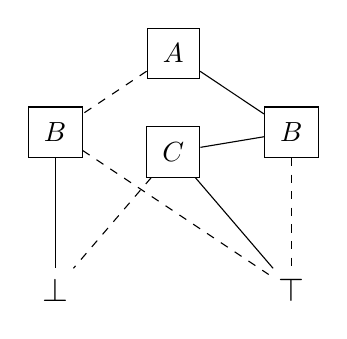
\begin{tikzpicture}
      \node[draw,inner sep=2mm] (a) at (0,0) {$A$};
      \node[draw,inner sep=2mm] (b1) at (-1.5, -1.0) {$B$};
      \node[draw,inner sep=2mm] (b2) at (1.5, -1.0) {$B$};
      \node[draw,inner sep=2mm] (c) at (0.0, -1.25) {$C$};
      \node (F) at (-1.5, -3.0) {\large$\bot$};
      \node (T) at (1.5, -3.0) {\large$\top$};
      \draw[dashed] (a) -- (b1);
      \draw (a) -- (b2);
      \draw[dashed] (b1) -- (T);
      \draw (b1) -- (F);
      \draw[dashed] (b2) -- (T);
      \draw (b2) -- (c);
      \draw[dashed] (c) -- (F);
      \draw (c) -- (T);
    \end{tikzpicture}
  \end{center}
  In their usual notation, inner nodes are variables and leaves are constants $\bot$ and $\top$.
  Evaluating an assignment $\set{x}\subseteq\{0,1\}^n$ is equivalent to a path from the root to a
  leaf where each variable $X$ determines a decision to go through the dashed line when $x=0$ or
  solid line when $x=1$. If the path ends at a $\top$, the function returns 1, otherwise it must
  end at a $\bot$ and therefore returns 0. The BDD above encodes the following logic formula
  \begin{equation*}
    \phi(A,B,C)=(A\vee\neg B)\wedge(\neg B\vee C),
  \end{equation*}
  also shown as a truth table on the right, together with a logic circuit that encodes the same
  truth table and its vtree.
  \tcblower
  \small%
  \begin{center}
    \begin{tabular}{ccc|c}
      \hline
      $A$ & $B$ & $C$ & $\phi(\set{x})$\\
      \hline
      0 & 0 & 0 & 1\\
      1 & 0 & 0 & 1\\
      0 & 1 & 0 & 0\\
      1 & 1 & 0 & 0\\
      0 & 0 & 1 & 1\\
      1 & 0 & 1 & 1\\
      0 & 1 & 1 & 0\\
      1 & 1 & 1 & 1\\
      \hline
    \end{tabular}

    Truth Table

    \begin{tikzpicture}
      \newOrNode[inputs=nn,fill=boxgreen]{r}{0,0};
      \newAndNode[inputs=nn,fill=boxred!70]{p1}{$(r) + (-1,-1)$};
      \newAndNode[inputs=nn,fill=boxred!70]{p2}{$(r) + (1,-1)$};
      \node (a) at ($(p1) + (-0.5,-1)$) {$A$};
      \newOrNode[inputs=nn,fill=boxpurple!60]{s1}{$(p1) + (0.5,-1)$};
      \node (na) at ($(p2) + (0.5,-1)$) {$\neg A$};
      \newAndNode[inputs=nn,fill=boxblue!80]{q1}{$(s1) + (-0.75,-1)$};
      \newAndNode[inputs=nn,fill=boxblue!80]{q2}{$(s1) + (0.75,-1)$};
      \newAndNode[inputs=nn,fill=boxblue!80]{q3}{$(p2.input 1) + (0,-1.75)$};
      \node (b) at ($(q1) + (-0.5,-1)$) {$B$};
      \node (c1) at ($(q1) + (0.5,-1)$) {$C$};
      \newOrNode[inputs=nn,fill=boxorange!80]{z1}{$(q2.input 1) + (0,-0.75)$};
      \node (nb) at ($(q3.input 2) + (0,-0.75)$) {$\neg B$};
      \node (c) at ($(z1) + (-0.5,-1)$) {$C$};
      \node (nc) at ($(z1) + (0.5,-1)$) {$\neg C$};
      \draw[edge] (r.input 1) -- ++(0,-0.2) -| (p1);
      \draw[edge] (r.input 2) -- ++(0,-0.2) -| (p2);
      \draw[edge] (s1.input 1) -- ++(0,-0.2) -| (q1);
      \draw[edge] (s1.input 2) -- ++(0,-0.2) -| (q2);
      \draw[edge] (p1.input 1) -- ++(0,-0.2) -| (a);
      \draw[edge] (p1.input 2) -- ++(0,-0.2) -| (s1);
      \draw[edge] (p2.input 1) -- (q3);
      \draw[edge] (p2.input 2) -- ++(0,-0.2) -| (na);
      \draw[edge] (q1.input 1) -- ++(0,-0.2) -| (b);
      \draw[edge] (q1.input 2) -- ++(0,-0.2) -| (c1);
      \draw[edge] (q2.input 1) -- (z1.east);
      \draw[edge] (q2.input 2) -- (nb.north);
      \draw[edge] (q3.input 1) -- (z1.east);
      \draw[edge] (q3.input 2) -- (nb.north);
      \draw[edge] (z1.input 1) -- ++(0,-0.2) -| (c);
      \draw[edge] (z1.input 2) -- ++(0,-0.2) -| (nc);
    \end{tikzpicture}

    \vskip -0.25cm
    Equivalent LC

    \begin{tikzpicture}
      \newVtreeNode{r}{0,0}{1};
      \newVtreeNode{l}{$(r) + (0.75,-1)$}{2};
      \node (x1) at ($(r) + (-0.75,-1)$) {$A$};
      \node (x2) at ($(l) + (-0.75,-1)$) {$B$};
      \node (x3) at ($(l) + (0.75,-1)$) {$C$};
      \draw (r) -- (l); \draw (r) -- (x1);
      \draw (l) -- (x2); \draw (l) -- (x3);
    \end{tikzpicture}

    \skip -0.35cm
    Vtree
  \end{center}
\end{example}

\subsection{...to Uncertainty}

Logic circuits are easily extensible to probabilistic circuits. In fact, if we think of an LC as
the support of a PC the connections between the two come naturally. Suppose a 2-standard smooth,
structure decomposable and deterministic probabilistic circuit $\mathcal{C}$ over binary variables.
We can construct an identically structured logic circuit (up to input nodes) $\mathcal{L}$ with
same vtree as $\mathcal{C}$ whose underlying Boolean function encodes $\phi(\set{x})=
\left\liv\mathcal{C}(\set{x})>0\right\riv$. Since sums act exactly like disjunctions and products
like conjunctions under the Boolean semiring, products in $\mathcal{L}$ are replaced with
conjunctions in $\mathcal{L}$, and sums with disjunctions. Input nodes from $\mathcal{C}$ are
replaced with a literal node if the function is degenerate, or with a disjunction over positive and
negative literals otherwise. This makes sure $\mathcal{L}$ acts as the support of $\mathcal{C}$, as
each disjunction node $\Sum_{\mathcal{L}}$ of $\mathcal{L}$ defines
\begin{equation*}
  \Sum_\mathcal{L}(\set{x})=\bigvee_{\Child\in\Ch_{\mathcal{C}}(\Sum_\mathcal{L})}\left\liv
  \Child_p(\set{x})>0\right\riv\wedge\left\liv\Child_s(\set{x})>0\right\riv,
\end{equation*}
where $\Ch_{\mathcal{C}}(\Sum)$ retrieves the children of $\Sum$'s corresponding sum node in
$\mathcal{C}$, with $\Child_p(\set{x})$ and $\Child_s(\set{x})$ the probabilities of $\Child$'s
prime and sub respectively. The corresponding sum node $\Sum_{\mathcal{C}}$ in $\mathcal{C}$ then
only attributes a weight (i.e.\ probability) to each positive element as usual
\begin{equation*}
  \Sum_\mathcal{C}(\set{x})=\sum_{\Child\in\Ch(\Sum_\mathcal{C})}w_{\Sum_\mathcal{C},\Child}\cdot
  \Child_p(\set{x})\cdot\Child_s(\set{x}).
\end{equation*}

\begin{example}[sidebyside,lefthand width=0.55\textwidth]{Embedding certain knowledge in probabilistic circuits}{pcsupp}

  Recall the logic circuit $\mathcal{L}$ from \Cref{eg:bdd}. Imagine we wish to model the
  uncertainty coming from all assignments where $\mathcal{L}(\set{x})=1$. In other words, we want
  to assign a positive probability to all true entries in the previous example's truth table,
  turning it into a probability table. The table on the right shows the chosen probabilities for
  each instance. Naturally, they all sum to one, with logically impossible assignments set to zero.

  Compiling an LC into a PC is straightforward: replace conjunctions with product nodes and
  disjunctions with sum nodes. Input nodes are left untouched, as literal nodes are just degenerate
  probability distributions. Sum weights are what ultimately define the probabilities in the
  probability table. The PC on the right is the result of the compilation of $\mathcal{L}$ into a
  probabilistic circuit whose distribution is defined by the probability table above it. When we
  mean to say that a PC has its support defined by its underlying LC, then we use the logic gate
  notation with the added weights on edges coming out from \inode{\newOrNode} nodes.

  \tcblower
  \small%
  \begin{center}
    \begin{tabular}{ccc|cc}
      \hline
      $A$ & $B$ & $C$ & $\phi(\set{x})$ & $p(\set{x})$\\
      \hline
      0 & 0 & 0 & 1 & 0.140\\
      1 & 0 & 0 & 1 & 0.024\\
      0 & 1 & 0 & 0 & \textcolor{gray}{0.000}\\
      1 & 1 & 0 & 0 & \textcolor{gray}{0.000}\\
      0 & 0 & 1 & 1 & 0.560\\
      1 & 0 & 1 & 1 & 0.096\\
      0 & 1 & 1 & 0 & \textcolor{gray}{0.000}\\
      1 & 1 & 1 & 1 & 0.180\\
      \hline
    \end{tabular}

    Probability Table

    \begin{tikzpicture}
      \newOrNode[inputs=nn,fill=boxgreen]{r}{0,0};
      \newAndNode[inputs=nn,fill=boxred!70]{p1}{$(r) + (-1,-1)$};
      \newAndNode[inputs=nn,fill=boxred!70]{p2}{$(r) + (1.5,-1)$};
      \node (a) at ($(p1) + (-0.5,-1)$) {$A$};
      \newOrNode[inputs=nn,fill=boxpurple!60]{s1}{$(p1) + (0.5,-1.25)$};
      \node (na) at ($(p2) + (0.5,-1)$) {$\neg A$};
      \newAndNode[inputs=nn,fill=boxblue!80]{q1}{$(s1) + (-0.75,-1)$};
      \newAndNode[inputs=nn,fill=boxblue!80]{q2}{$(s1) + (0.75,-1)$};
      \newAndNode[inputs=nn,fill=boxblue!80]{q3}{$(p2.input 1) + (0,-2.0)$};
      \node (b) at ($(q1) + (-0.5,-1)$) {$B$};
      \node (c1) at ($(q1) + (0.5,-1)$) {$C$};
      \newOrNode[inputs=nn,fill=boxorange!80]{z1}{$(q2.input 1) + (0,-1.0)$};
      \node (nb) at ($(q3.input 2) + (0,-1.0)$) {$\neg B$};
      \node (c) at ($(z1) + (-0.5,-1)$) {$C$};
      \node (nc) at ($(z1) + (0.5,-1)$) {$\neg C$};
      \draw[edge] (r.input 1) -- ++(0,-0.2) -| node[near start,above left] {$0.3$} (p1);
      \draw[edge] (r.input 2) -- ++(0,-0.2) -| node[near start,above right] {$0.7$} (p2);
      \draw[edge] (s1.input 1) -- ++(0,-0.2) -| node[near start,above left] {$0.6$} (q1);
      \draw[edge] (s1.input 2) -- ++(0,-0.2) -| node[near start,above right] {$0.4$} (q2);
      \draw[edge] (p1.input 1) -- ++(0,-0.2) -| (a);
      \draw[edge] (p1.input 2) -- ++(0,-0.2) -| (s1);
      \draw[edge] (p2.input 1) -- (q3);
      \draw[edge] (p2.input 2) -- ++(0,-0.2) -| (na);
      \draw[edge] (q1.input 1) -- ++(0,-0.2) -| (b);
      \draw[edge] (q1.input 2) -- ++(0,-0.2) -| (c1);
      \draw[edge] (q2.input 1) -- (z1.east);
      \draw[edge] (q2.input 2) -- (nb.north);
      \draw[edge] (q3.input 1) -- (z1.east);
      \draw[edge] (q3.input 2) -- (nb.north);
      \draw[edge] (z1.input 1) -- ++(0,-0.2) -| node[near start,above left] {$0.8$} (c);
      \draw[edge] (z1.input 2) -- ++(0,-0.2) -| node[near start,above right] {$0.2$} (nc);
    \end{tikzpicture}

    \vskip -0.25cm
    Probabilistic Circuit
  \end{center}
\end{example}

This compatibility between logic and probabilistic circuits allows certain knowledge to be embedded
into an uncertain model by constructing a computational graph whose underlying logic circuit
correctly attributes positive values only to the support of the distribution. An alternative use
case for logic circuits within the context of probabilistic reasoning is querying for the
probability of logical events, i.e.\ the expectation of a logic query with respect to a
distribution. This kind of query is enabled by the following result.

\begin{algorithm}[t]
  \caption{\expc}\label{alg:expc}
  \begin{algorithmic}[1]
    \Require A smooth, structure decomposable PC $\mathcal{C}$ and LC $\mathcal{L}$ both with vtree
      $\vtree$
    \Ensure The expectation $\mathbb{E}_\mathcal{C}\left[\mathcal{L}\right]=\int\mathcal{C}(\set{x})
      \mathcal{L}(\set{x})\dif\set{x}$
    \State Let $v$ a hash function mapping a node to its expectation
    \For{each pair of nodes $(\Node_\mathcal{C},\Node_\mathcal{L})$ in reverse topological order}\label{alg:expc:line:top}
      \IIf{$\Node_\mathcal{C}$ is an input}{$v_{\Node_\mathcal{C}}\gets
        \mathbb{E}_{\Node_\mathcal{C}}\left[\Node_\mathcal{L}\right]$}
      \IElseIf{$\Node_\mathcal{C}$ is a product}{$v_{\Node_\mathcal{C}}\gets
        \prod_{\Child\in\Ch(\Node_\mathcal{C})}v_{\Child}$}
      \IElseIf{$\Node_\mathcal{C}$ is a sum}{$v_{\Node_\mathcal{C}}\gets
        \sum_{\Child'\in\Ch(\Node_\mathcal{C})}\sum_{\Child''\in\Ch(\Node_\mathcal{L})}
        w_{\Sum,\Child'}\cdot v_{\Node_{\Child'}}$}%
    \EndFor%
    \State \textbf{return} $v_R$, where $\textsf{R}$ is $\mathcal{C}$'s root
  \end{algorithmic}
\end{algorithm}

\begin{restatable}[\cite{choi20}]{theorem}{expc}
  If $\mathcal{C}$ is a smooth and structure decomposable probabilistic circuit with vtree
  $\vtree$, and $\mathcal{L}$ a structure decomposable logic circuit also respecting $\vtree$, then
  $\mathbb{E}_\mathcal{C}\left[\mathcal{L}\right]$ is polynomial time computable (in the number of
  edges).
\end{restatable}

Let $\mathcal{C}$ a smooth and structure decomposable circuit with vtree $\vtree$, and
$\mathcal{L}$ a logic circuit representing a logical query whose vtree is also $\vtree$. Computing
the probability of $\mathcal{L}$ with respect to the distribution encoded by $\mathcal{C}$ is done
by a bottom-up evaluation over both circuits at the same time. \Cref{alg:expc} shows the procedure
algorithmically. Importantly, the procedure relies on evaluating the expectation for each node in
a reverse topological fashion according to \ref{alg:expc:line:top}. This paired reverse
topological sorting is done by a recursive assignment. For product nodes, primes are paired with
primes, and subs with subs; for sums, each combination of PC child with LC child is paired up.

\begin{example}[sidebyside,lefthand width=0.55\textwidth]{Computing the probability of logical events}{problog}
\tcblower

\end{example}
